\documentclass[a4paper,12pt,twoside]{memoir}

% Castellano
\usepackage[spanish,es-tabla]{babel}
\selectlanguage{spanish}
\usepackage[utf8]{inputenc}
\usepackage[T1]{fontenc}
\usepackage{lmodern} % scalable font
\usepackage{microtype}
\usepackage{placeins}

\RequirePackage{booktabs}
\RequirePackage[table]{xcolor}
\RequirePackage{xtab}
\RequirePackage{multirow}

% Links
\PassOptionsToPackage{hyphens}{url}\usepackage[colorlinks]{hyperref}
\hypersetup{
	allcolors = {red}
}

% Ecuaciones
\usepackage{amsmath}

% Landscape
\usepackage{pdflscape}

% Rutas de fichero / paquete
\newcommand{\ruta}[1]{{\sffamily #1}}

% Párrafos
\nonzeroparskip

% Huérfanas y viudas
\widowpenalty100000
\clubpenalty100000

% Evitar solapes en el header
\nouppercaseheads

% Imagenes
\usepackage{graphicx}
\newcommand{\imagen}[2]{
	\begin{figure}[!h]
		\centering
		\includegraphics[width=0.9\textwidth]{#1}
		\caption{#2}\label{fig:#1}
	\end{figure}
	\FloatBarrier
}

\newcommand{\imagenflotante}[2]{
	\begin{figure}%[!h]
		\centering
		\includegraphics[width=0.9\textwidth]{#1}
		\caption{#2}\label{fig:#1}
	\end{figure}
}



% El comando \figura nos permite insertar figuras comodamente, y utilizando
% siempre el mismo formato. Los parametros son:
% 1 -> Porcentaje del ancho de página que ocupará la figura (de 0 a 1)
% 2 --> Fichero de la imagen
% 3 --> Texto a pie de imagen
% 4 --> Etiqueta (label) para referencias
% 5 --> Opciones que queramos pasarle al \includegraphics
% 6 --> Opciones de posicionamiento a pasarle a \begin{figure}
\newcommand{\figuraConPosicion}[6]{%
  \setlength{\anchoFloat}{#1\textwidth}%
  \addtolength{\anchoFloat}{-4\fboxsep}%
  \setlength{\anchoFigura}{\anchoFloat}%
  \begin{figure}[#6]
    \begin{center}%
      \Ovalbox{%
        \begin{minipage}{\anchoFloat}%
          \begin{center}%
            \includegraphics[width=\anchoFigura,#5]{#2}%
            \caption{#3}%
            \label{#4}%
          \end{center}%
        \end{minipage}
      }%
    \end{center}%
  \end{figure}%
}

%
% Comando para incluir imágenes en formato apaisado (sin marco).
\newcommand{\figuraApaisadaSinMarco}[5]{%
  \begin{figure}%
    \begin{center}%
    \includegraphics[angle=90,height=#1\textheight,#5]{#2}%
    \caption{#3}%
    \label{#4}%
    \end{center}%
  \end{figure}%
}
% Para las tablas
\newcommand{\otoprule}{\midrule [\heavyrulewidth]}
%
% Nuevo comando para tablas pequeñas (menos de una página).
\newcommand{\tablaSmall}[5]{%
 \begin{table}
  \begin{center}
   \rowcolors {2}{gray!35}{}
   \begin{tabular}{#2}
    \toprule
    #4
    \otoprule
    #5
    \bottomrule
   \end{tabular}
   \caption{#1}
   \label{tabla:#3}
  \end{center}
 \end{table}
}

%
%Para el float H de tablaSmallSinColores
\usepackage{float}

%
% Nuevo comando para tablas pequeñas (menos de una página).
\newcommand{\tablaSmallSinColores}[5]{%
 \begin{table}[H]
  \begin{center}
   \begin{tabular}{#2}
    \toprule
    #4
    \otoprule
    #5
    \bottomrule
   \end{tabular}
   \caption{#1}
   \label{tabla:#3}
  \end{center}
 \end{table}
}

\newcommand{\tablaApaisadaSmall}[5]{%
\begin{landscape}
  \begin{table}
   \begin{center}
    \rowcolors {2}{gray!35}{}
    \begin{tabular}{#2}
     \toprule
     #4
     \otoprule
     #5
     \bottomrule
    \end{tabular}
    \caption{#1}
    \label{tabla:#3}
   \end{center}
  \end{table}
\end{landscape}
}

%
% Nuevo comando para tablas grandes con cabecera y filas alternas coloreadas en gris.
\newcommand{\tabla}[6]{%
  \begin{center}
    \tablefirsthead{
      \toprule
      #5
      \otoprule
    }
    \tablehead{
      \multicolumn{#3}{l}{\small\sl continúa desde la página anterior}\\
      \toprule
      #5
      \otoprule
    }
    \tabletail{
      \hline
      \multicolumn{#3}{r}{\small\sl continúa en la página siguiente}\\
    }
    \tablelasttail{
      \hline
    }
    \bottomcaption{#1}
    \rowcolors {2}{gray!35}{}
    \begin{xtabular}{#2}
      #6
      \bottomrule
    \end{xtabular}
    \label{tabla:#4}
  \end{center}
}

%
% Nuevo comando para tablas grandes con cabecera.
\newcommand{\tablaSinColores}[6]{%
  \begin{center}
    \tablefirsthead{
      \toprule
      #5
      \otoprule
    }
    \tablehead{
      \multicolumn{#3}{l}{\small\sl continúa desde la página anterior}\\
      \toprule
      #5
      \otoprule
    }
    \tabletail{
      \hline
      \multicolumn{#3}{r}{\small\sl continúa en la página siguiente}\\
    }
    \tablelasttail{
      \hline
    }
    \bottomcaption{#1}
    \begin{xtabular}{#2}
      #6
      \bottomrule
    \end{xtabular}
    \label{tabla:#4}
  \end{center}
}

%
% Nuevo comando para tablas grandes sin cabecera.
\newcommand{\tablaSinCabecera}[5]{%
  \begin{center}
    \tablefirsthead{
      \toprule
    }
    \tablehead{
      \multicolumn{#3}{l}{\small\sl continúa desde la página anterior}\\
      \hline
    }
    \tabletail{
      \hline
      \multicolumn{#3}{r}{\small\sl continúa en la página siguiente}\\
    }
    \tablelasttail{
      \hline
    }
    \bottomcaption{#1}
  \begin{xtabular}{#2}
    #5
   \bottomrule
  \end{xtabular}
  \label{tabla:#4}
  \end{center}
}



\definecolor{cgoLight}{HTML}{EEEEEE}
\definecolor{cgoExtralight}{HTML}{FFFFFF}

%
% Nuevo comando para tablas grandes sin cabecera.
\newcommand{\tablaSinCabeceraConBandas}[5]{%
  \begin{center}
    \tablefirsthead{
      \toprule
    }
    \tablehead{
      \multicolumn{#3}{l}{\small\sl continúa desde la página anterior}\\
      \hline
    }
    \tabletail{
      \hline
      \multicolumn{#3}{r}{\small\sl continúa en la página siguiente}\\
    }
    \tablelasttail{
      \hline
    }
    \bottomcaption{#1}
    \rowcolors[]{1}{cgoExtralight}{cgoLight}

  \begin{xtabular}{#2}
    #5
   \bottomrule
  \end{xtabular}
  \label{tabla:#4}
  \end{center}
}




\graphicspath{ {./img/} }

% Capítulos
\chapterstyle{bianchi}
\newcommand{\capitulo}[2]{
	\setcounter{chapter}{#1}
	\setcounter{section}{0}
	\setcounter{figure}{0}
	\setcounter{table}{0}
	\chapter*{#2}
	\addcontentsline{toc}{chapter}{#2}
	\markboth{#2}{#2}
}

% Apéndices
\renewcommand{\appendixname}{Apéndice}
\renewcommand*\cftappendixname{\appendixname}

\newcommand{\apendice}[1]{
	%\renewcommand{\thechapter}{A}
	\chapter{#1}
}

\renewcommand*\cftappendixname{\appendixname\ }

% Formato de portada
\makeatletter
\usepackage{xcolor}
\newcommand{\tutor}[1]{\def\@tutor{#1}}
\newcommand{\course}[1]{\def\@course{#1}}
\definecolor{cpardoBox}{HTML}{E6E6FF}
\def\maketitle{
  \null
  \thispagestyle{empty}
  % Cabecera ----------------
\noindent
\includegraphics[width=\textwidth]{cabecera}\vspace{1cm}%
  \vfill
  % Título proyecto y escudo informática ----------------
  \colorbox{cpardoBox}{%
    \begin{minipage}{.8\textwidth}
      \vspace{.5cm}\Large
      \begin{center}
      \textbf{TFG del Grado en Ingeniería Informática}\vspace{.6cm}\\
      \textbf{\LARGE\@title{}}
      \end{center}
      \vspace{.2cm}
    \end{minipage}

  }%
  \hfill\begin{minipage}{.20\textwidth}
    
\includegraphics[width=\textwidth]{escudoInfor}
  \end{minipage}
  \vfill
  % Datos de alumno, curso y tutores ------------------
  \begin{center}%
  {%
    \noindent\LARGE
    Presentado por \@author{}\\ 
    en Universidad de Burgos --- \@date{}\\
    Tutores: \@tutor{}\\
  }%
  \end{center}%
  \null
  \cleardoublepage
  }
\makeatother

\newcommand{\nombre}{Ahmad Mareie Pascual}
\newcommand{\nombreTutorA}{José Manuel Aroca Fernández}
\newcommand{\nombreTutorB}{Jesús Manuel Maudes Raedo}

% Datos de portada
\title{{\Huge ReservApp}\\[0.5cm]Aplicación para la Gestión de Reservas\\Documentación Técnica}
\author{\nombre}
\tutor{D. {\nombreTutorA} \\y Dr. {\nombreTutorB}}
\date{\today}

\begin{document}

\maketitle



\cleardoublepage



%%%%%%%%%%%%%%%%%%%%%%%%%%%%%%%%%%%%%%%%%%%%%%%%%%%%%%%%%%%%%%%%%%%%%%%%%%%%%%%%%%%%%%%%



\frontmatter


\clearpage

% Indices
\tableofcontents

\clearpage

\listoffigures

\clearpage

\listoftables

\clearpage

\mainmatter

\appendix

\apendice{Plan de Proyecto Software}

\section{Introducción}
En el presente plan de proyecto se define la estrategia de desarrollo mediante la cual se ha llevado a cabo la implementación de un sistema web de gestión de reservas de salas de reuniones. Este anexo establece el marco organizativo y metodológico que se llevó a cabo durante el proceso de desarrollo, desde la concepción inicial hasta la puesta en producción del sistema. La planificación aquí presentada contempla una estimación temporal realista de las diferentes fases del proyecto, considerando las actividades de análisis, diseño, implementación, pruebas y despliegue. Asimismo, se evalúa la viabilidad del proyecto desde una perspectiva económica y legal, analizando los costes asociados al desarrollo, los recursos necesarios y el cumplimiento de la normativa aplicable en materia de protección de datos y propiedad intelectual.

\section{Planificación temporal}
Para el desarrollo de la aplicación de gestión de reservas de salas de reuniones se ha adoptado la metodología ágil Scrum como marco de trabajo principal. Esto ha sido debido a que Scrum, por la naturaleza iterativa e incremental, permite que el proyecto se adapte en cualquier momento a los requisitos cambiantes y una entrega de valor constante a lo largo del proceso de desarrollo.

Scrum proporciona un marco estructurado que facilita la organización del trabajo en iteraciones cortas llamadas sprints, que se realizan normalmente en un periodo de de 2 semanas de duración. Scrum permite una mayor flexibilidad en la gestión de cambios, una mejor comunicación con los tutores y una entrega más predecible de funcionalidades. Además, la transparencia inherente a Scrum facilita la identificación temprana de impedimentos y riesgos, permitiendo su resolución antes de que impacten significativamente en el proyecto.

La gestión y seguimiento de los sprints se ha realizado utilizando Zube~\cite{zube}, que es una plataforma especializada en la gestión de proyectos ágiles y que se integra perfectamente con el repositorio de GitHub. Además, Zube ofrece funcionalidades específicas para la implementación de Scrum, que incluyen:

\begin{itemize}
\tightlist
\item
\textbf{Tableros Kanban personalizables}: Permiten visualizar el flujo de trabajo desde el backlog hasta la finalización de las tareas. Como ejemplo de ello se puede observa la figura ~\ref{fig:Zube-Kanban}
\item

\imagen{Zube-Kanban}{Ejemplo de las tarjetas de un sprint en Zube con los diferentes estados en los que se puede encontrar.}{1.0}

\textbf{Gestión de sprints}: Dispone de herramientas para la planificación, seguimiento y retrospectivas de cada iteración.
\item
\textbf{Métricas de rendimiento}: Incluyen gráficos de \emph{burndown charts}, \emph{velocity tracking} y análisis de ciclo de vida de las tareas. En la figura ~\ref{fig:Zube-Burndown} se puede observar un ejemplo de gráfica de \emph{burndown}.

\imagen{Zube-Burndown}{Ejemplo de gráfico de \emph{burndown} en el que se muestra la evolución de los puntos realizados.}{1.0}

\item
\textbf{Integración nativa con GitHub}: Permite la sincronización automática con \emph{issues}, \emph{pull requests} y \emph{commits}.
\end{itemize}

La elección de Zube se justifica por su capacidad de proporcionar una visión global del progreso del proyecto, facilitando con ello tanto la planificación a corto plazo como el seguimiento de objetivos a largo plazo. Su interfaz es intuitiva y permite una gestión eficiente del \emph{product backlog} y la asignación de tareas a cada sprint.

Complementariamente al uso de Zube, se ha utilizado el sistema de issues de GitHub para el registro detallado de todas las tareas, errores, mejoras y funcionalidades del proyecto. Esta integración dual proporciona varios beneficios:

\begin{itemize}
\tightlist
\item
\textbf{Trazabilidad completa}: Cada \emph{issue} está vinculada directamente con el código fuente, \emph{commits} y \emph{pull requests} correspondientes. En la figura ~\ref{fig:GitHub-Issue3} se puede observar un ejemplo del histórico de una \emph{issue}.
\item
\textbf{Documentación técnica}: Los \emph{issues} permiten documentar decisiones técnicas, problemas encontrados y soluciones implementadas.
\item
\textbf{Colaboración eficiente}: Facilita la comunicación sobre aspectos técnicos específicos y la revisión de código.
\item
\textbf{Historial detallado}: Mantiene un registro completo de la evolución del proyecto y las decisiones tomadas.
\end{itemize}

\imagen{GitHub-Issue3}{Ejemplo del histórico de una \emph{issue}.}{1.0}

\subsection{Estructura y Duración del Proyecto}
El proyecto se ha estructurado en 10 sprints de 2 semanas cada uno, resultando en una duración total de 20 semanas (aproximadamente 5 meses). Esta planificación se ha diseñado considerando la complejidad del sistema a desarrollar y los recursos disponibles, permitiendo un desarrollo incremental y sostenible.

Cabe señalar que la distribución temporal del proyecto no ha seguido un patrón estrictamente lineal debido a interrupciones planificadas relacionadas con el calendario académico que ha requerido pausas en el desarrollo del proyecto, adaptando la planificación a las exigencias del curso académico. Esta variabilidad temporal ha sido gestionada mediante la flexibilidad que ofrece la metodología Scrum, permitiendo ajustar la duración de algunos sprints y redistribuir las cargas de trabajo según la disponibilidad. A pesar de estas interrupciones, se ha mantenido la estructura de 10 sprints planificada, asegurando que los objetivos de cada iteración se cumplieran independientemente de las fluctuaciones en el ritmo de trabajo, quédando resumida la planificación en los siguientes puntos:

\begin{itemize}
\tightlist
\item
\textbf{Duración total del proyecto}: 20 semanas.
\item
\textbf{Número de sprints}: 10.
\item
\textbf{Duración de cada sprint}: 2 semanas.
\item
\textbf{Eventos Scrum}: Planificación de sprint, \emph{daily standups}, revisión y retrospectiva.
\item
\textbf{Período de desarrollo activo}: 17 semanas.
\item
\textbf{Período de cierre y documentación}: 3 semanas.
\end{itemize}

\subsection{Detalle de los Sprints}

\subsubsection{Sprint 0 - Configuración Inicial y Arquitectura Base (17/03/2025 – 30/03/2025)} 
En este sprint inicial se establecieron los cimientos del proyecto ReservApp como aplicación web para gestión de reservas. Se configuró el entorno de desarrollo con Spring Boot 3.4.4 como framework principal, estableciendo una arquitectura basada en capas (presentación, servicio, persistencia). Se configuró la estructura Maven con gestión de dependencias optimizada, incluyendo Spring Data JPA para persistencia, Spring Security para autenticación, Thymeleaf como motor de templates y MySQL como base de datos principal. En esta configuración inicial se priorizó la escalabilidad y mantenibilidad, preparando el proyecto para futuras ampliaciones mediante Docker Compose y herramientas de calidad continua como SonarCloud y JaCoCo para análisis de cobertura de código.

Objetivos principales:
\begin{itemize}
\tightlist
\item
Configurar proyecto Spring Boot con Maven.
\item
Establecer arquitectura en capas (controller, service, repository, model).
\item
Configurar base de datos MySQL con pool de conexiones.
\item
Implementar configuración de desarrollo con Docker Compose.
\item
Establecer herramientas de calidad de código (SonarCloud, JaCoCo).
\end{itemize}

Actividades realizadas:
\begin{itemize}
\tightlist
\item
Creación del 'pom.xml' con todas las dependencias necesarias.
\item
Configuración de `application.properties` con parámetros de BD y logging.
\item
Estructura de paquetes modular: 'controller', 'service', 'model', 'config'.
\item
Configuración de 'compose.yaml' para contenedores de desarrollo.
\item
Integración con SonarCloud mediante 'sonar-project.properties' para análisis continuo.
\item
Implementación de 'ReservApplication' como clase principal con configuración de componentes
\end{itemize}


\subsubsection{Sprint 1 - Modelo de Datos y Entidades Base (31/03/2025 – 13/04/2025)} 
En este sprint se diseñó e implementó el modelo de datos completo del sistema, creando las entidades principales que sustentan la funcionalidad de reservas. Se desarrolló una jerarquía de entidades con 'EntidadInfo' como clase base que proporciona auditoría automática, y se implementaron las entidades principales: 'Usuario', 'Establecimiento', 'Reserva', 'Perfil' y 'Menu'. Se establecieron las relaciones entre entidades usando JPA annotations, implementando validaciones con Bean Validation y configurando índices de base de datos para optimizar las consultas más frecuentes. También se creó el sistema de claves primarias personalizadas con 'EntidadPK' y 'EntidadID'.

Objetivos principales:
\begin{itemize}
\tightlist
\item
Diseñar modelo de datos completo del sistema.
\item
Implementar entidades JPA con validaciones.
\item
Establecer relaciones entre entidades.
\item
Configurar sistema de auditoría automática con interceptores de entidad personalizados.
\item
Optimizar consultas con índices de base de datos.
\end{itemize}

Actividades realizadas:
\begin{itemize}
\tightlist
\item
Creación de 'EntidadInfo' como clase base con auditoría.
\item
Implementación de entidades: 'Usuario', 'Establecimiento', 'Reserva'.
\item
Desarrollo de 'Perfil' y 'Menu' para gestión de perfiles.
\item
Configuración de relaciones '@OneToMany', '@ManyToMany', '@ManyToOne'.
\item
Implementación de validaciones con '@NotNull', '@Email', '@Pattern'.
\end{itemize}

\subsubsection{Sprint 2 - Seguridad y Autenticación (14/04/2025 – 27/04/2025)} 
Este sprint se centró en implementar un sistema de seguridad robusto utilizando Spring Security y, para ello, se desarrolló un sistema de autenticación personalizado con 'CustomUserDetailsService' y 'CustomAuthenticationSuccessHandler', implementando encriptación de contraseñas con BCrypt y control de acceso basado en roles (USER/ADMIN). Se configuró la seguridad web con páginas de login personalizadas, protección contra ataques comunes (CSRF, session fixation, clickjacking) y manejo de sesiones. También se implementó el sistema de registro de usuarios con validación de email y tokens de confirmación, y se estableció un sistema de gestión de sesiones con timeout configurable y logout seguro.

Objetivos principales:
\begin{itemize}
\tightlist
\item
Implementar autenticación con Spring Security.
\item
Crear sistema de roles y permisos.
\item
Desarrollar páginas de login y registro personalizadas.
\item
Configurar encriptación de contraseñas.
\item
Implementar control de sesiones y logout
\end{itemize}

Actividades realizadas:
\begin{itemize}
\tightlist
\item
Desarrollo de 'SecurityConfig' con configuración completa.
\item
Creación de 'CustomUserDetailsService' para carga de usuarios.
\item
Implementación de 'CustomAuthenticationSuccessHandler'.
\item
Desarrollo de 'LoginController' con registro y autenticación.
\item
Creación de templates 'login.html' y 'registro.html'
\end{itemize}

\subsubsection{Sprint 3 - Gestión de Usuarios y Perfiles (28/04/2025 – 11/05/2025)} 
En este sprint se desarrolló la funcionalidad completa de gestión de usuarios y perfiles del sistema. Se implementaron los servicios 'UsuarioService' y 'PerfilService' con operaciones CRUD completas, incluyendo funcionalidades avanzadas como búsqueda de usuarios, asignación de establecimientos y gestión de perfiles personalizados. Se creó el panel de administración para gestión de usuarios con capacidades de bloqueo/desbloqueo, edición de perfiles y asignación de roles. También se implementó la funcionalidad de edición de perfil personal y la gestión de menús asociados a perfiles, estableciendo la base para un sistema de permisos granular.

Objetivos principales:
\begin{itemize}
\tightlist
\item
Desarrollar CRUD completo para usuarios.
\item
Implementar gestión de perfiles personalizados.
\item
Crear panel de administración de usuarios.
\item
Desarrollar funcionalidad de búsqueda y filtrado.
\item
Implementar asignación de establecimientos a usuarios
\end{itemize}

Actividades realizadas:
\begin{itemize}
\tightlist
\item
Implementación de 'UsuarioServiceImpl' con operaciones completas.
\item
Desarrollo de 'PerfilServiceImpl' y gestión de menús.
\item
Creación de 'UserManagementController' para administración.
\item
Desarrollo de 'EditarPerfilController' para usuarios.
\item
Implementación de templates de gestión de usuarios y perfiles
\end{itemize}

\subsubsection{Sprint 4 - Gestión de Establecimientos (09/06/2025 – 22/07/2025)} 
Este sprint se enfocó en desarrollar el módulo completo de gestión de establecimientos, implementando funcionalidades para crear, editar y administrar los espacios disponibles para reservas. Se desarrolló el sistema de franjas horarias con 'FranjaHoraria' que permite definir horarios de apertura por día de la semana, y se implementó la lógica de aforo para controlar la capacidad máxima de reservas simultáneas. Se creó la funcionalidad de asignación de establecimientos a usuarios, permitiendo que cada usuario tenga acceso solo a los establecimientos autorizados. También se implementaron validaciones de negocio para asegurar la consistencia de los datos de establecimientos.

Objetivos principales:
\begin{itemize}
\tightlist
\item
Desarrollar CRUD completo para establecimientos.
\item
Implementar sistema de franjas horarias.
\item
Crear funcionalidad de aforo y capacidad.
\item
Desarrollar asignación de usuarios a establecimientos.
\item
Implementar validaciones de negocio específicas
\end{itemize}

Actividades realizadas:
\begin{itemize}
\tightlist
\item
Implementación de 'EstablecimientoServiceImpl' con lógica completa.
\item
Desarrollo de 'EstablecimientoController' y 'EstablecimientoAsignacionController'.
\item
Creación de entidad 'FranjaHoraria' con relaciones.
\item
Implementación de templates para gestión de establecimientos.
\item
Desarrollo de funcionalidad de asignación usuario-establecimiento.
\end{itemize}







\subsubsection{Sprint 5 - Sistema de Reservas Core (23/06/2025 – 06/07/2025)} 
En este sprint se desarrolló el núcleo del sistema de reservas, implementando la lógica completa para crear, modificar y gestionar reservas. Se creó 'ReservaService' con algoritmos sofisticados para verificar disponibilidad considerando aforo, franjas horarias y conflictos de tiempo. Se implementó el sistema de slots de tiempo con 'SlotReservaUtil' que genera automáticamente los horarios disponibles basados en la configuración del establecimiento. Se desarrolló la funcionalidad de calendario interactivo que permite a los usuarios visualizar y seleccionar fechas y horarios disponibles. También se implementó la lógica de validación de reservas que considera múltiples factores como horarios de apertura, aforo máximo y reservas existentes.

Objetivos principales:
\begin{itemize}
\tightlist
\item
Desarrollar lógica core de reservas.
\item
Implementar algoritmos de verificación de disponibilidad.
\item
Crear sistema de slots de tiempo automático.
\item
Desarrollar calendario interactivo de reservas.
\item
Implementar validaciones complejas de negocio.
\end{itemize}

Actividades realizadas:
\begin{itemize}
\tightlist
\item
Implementación de 'ReservaServiceImpl' con lógica avanzada.
\item
Desarrollo de 'SlotReservaUtil' para generación de slots.
\item
Creación de algoritmos de verificación de aforo.
\item
Implementación de 'ReservaController' con validaciones.
\item
Desarrollo de templates de calendario y gestión de reservas.
\end{itemize}

\subsubsection{Sprint 6 - Sistema de Convocatorias (07/07/2025 – 20/07/2025)} 
Este sprint se centró en desarrollar el sistema de convocatorias que permite invitar a otros usuarios a las reservas creadas. Se implementaron las entidades 'Convocatoria' y 'Convocado' con una relación compleja que maneja claves primarias compuestas mediante 'ConvocadoPK'. Se desarrolló la funcionalidad de búsqueda de usuarios para invitaciones, implementando un sistema AJAX que permite buscar y seleccionar usuarios dinámicamente. Se creó el sistema de notificaciones por email que informa a los usuarios convocados sobre las reservas, incluyendo detalles como fecha, hora, establecimiento y enlaces de reunión. También se implementó la gestión de convocatorias con capacidades de edición y eliminación.

Objetivos principales:
\begin{itemize}
\tightlist
\item
Desarrollar sistema completo de convocatorias.
\item
Implementar búsqueda dinámica de usuarios.
\item
Crear sistema de notificaciones por email.
\item
Desarrollar gestión de usuarios convocados.
\item
Implementar funcionalidad de enlaces de reunión.
\end{itemize}

Actividades realizadas:
\begin{itemize}
\tightlist
\item
Implementación de entidades 'Convocatoria' y 'Convocado'.
\item
Desarrollo de 'ConvocatoriaService' con lógica compleja.
\item
Creación de sistema de búsqueda AJAX de usuarios.
\item
Implementación de 'EmailService' para notificaciones.
\item
Desarrollo de funcionalidades de gestión de convocatorias.
\end{itemize}


\subsubsection{Sprint 7 - Interfaz de Usuario y Experiencia (04/08/2025 – 17/08/2025)} 
En este sprint se desarrolló una interfaz de usuario moderna y responsiva utilizando Bootstrap y componentes personalizados. Se creó el sistema de templates con Thymeleaf, implementando fragmentos reutilizables como '_header.html' y '_common_head.html' para mantener consistencia visual. Se desarrolló el menú principal dinámico que adapta las opciones disponibles según el rol del usuario (USER/ADMIN), y se implementaron interfaces específicas para cada funcionalidad del sistema. Se creó un sistema de mensajes flash para feedback del usuario y se implementaron validaciones del lado cliente con JavaScript. También se optimizó la experiencia móvil con diseño responsivo.

Objetivos principales:
\begin{itemize}
\tightlist
\item
Desarrollar interfaz moderna con Bootstrap.
\item
Crear sistema de templates reutilizables.
\item
Implementar diseño responsivo para móviles.
\item
Desarrollar componentes JavaScript interactivos.
\item
Crear sistema de feedback visual para usuarios.
\end{itemize}

Actividades realizadas:
\begin{itemize}
\tightlist
\item
Implementación de templates Thymeleaf con fragmentos.
\item
Desarrollo de `menuprincipal.html` con navegación dinámica.
\item
Creación de estilos CSS personalizados.
\item
Implementación de componentes JavaScript para interactividad.
\item
Desarrollo de interfaces específicas para cada módulo.
\end{itemize}

\subsubsection{Sprint 8 - Funcionalidades Avanzadas y Optimizaciones (18/08/2025 – 31/08/2025)} 

Objetivos principales:
\begin{itemize}
\tightlist
\item
Desarrollar .
\item
Implementar.
\item
Crear.
\item
Desarrollar.
\item
Implementar.
\end{itemize}

Actividades realizadas:
\begin{itemize}
\tightlist
\item
Implementación.
\item
Desarrollo.
\item
Creación.
\item
Implementación.
\item
Desarrollo
\end{itemize}

\subsubsection{Sprint 9 - Testing, Documentación y Despliegue (01/09/2025 – 14/09/2025)} 

Objetivos principales:
\begin{itemize}
\tightlist
\item
Desarrollar .
\item
Implementar.
\item
Crear.
\item
Desarrollar.
\item
Implementar.
\end{itemize}

Actividades realizadas:
\begin{itemize}
\tightlist
\item
Implementación.
\item
Desarrollo.
\item
Creación.
\item
Implementación.
\item
Desarrollo
\end{itemize}








\section{Estudio de viabilidad}


\subsection{Viabilidad económica}


\subsection{Viabilidad legal}



\apendice{Especificación de Requisitos}

\section{Introducción}
Este documento presenta la especificación completa de requisitos para ReservApp, un sistema web de gestión de reservas. El objetivo es definir de manera precisa y detallada las funcionalidades, características técnicas y restricciones del sistema, proporcionando una base sólida para el desarrollo, testing y mantenimiento de la aplicación.

ReservApp es una aplicación web diseñada para facilitar la gestión integral de reservas en establecimientos diversos. El sistema permite a los usuarios realizar reservas en diferentes establecimientos, gestionar convocatorias con otros usuarios, y a los administradores supervisar todo el proceso de reservas y gestión de usuarios.

\section{Objetivos generales}

El objetivo principal del actual TFG es el desarrollo de un sistema web de gestión de reservas que permita a los usuarios realizar reservas de manera eficiente en diferentes establecimientos, con capacidades avanzadas de convocatorias y administración centralizada. Y como consecuencia de ello, se deben contemplar los siguientes objetivos específicos:

\begin{itemize}
\tightlist
\item
Gestión de Establecimientos.
    \begin{itemize}
    \tightlist
    \item
    Permitir la configuración flexible de establecimientos con horarios específicos.
    \item
    Implementar sistema de aforo para controlar la capacidad de reservas.
    \item
    Proporcionar asignación de usuarios a establecimientos específicos.
    \item
    Facilitar la gestión administrativa de establecimientos.
    \end{itemize}

\item
Gestión de Usuarios.
    \begin{itemize}
    \tightlist
    \item
    Proporcionar un sistema de registro y autenticación seguro.
    \item
    Implementar control de acceso basado en roles (Usuario/Administrador).
    \item
    Permitir la gestión de perfiles de usuario personalizables.
    \end{itemize}

\item
Sistema de Reservas.
    \begin{itemize}
    \tightlist
    \item
    Ofrecer múltiples modalidades de reserva (slots predefinidos y horarios libres).
    \item
    Implementar validación automática de disponibilidad y conflictos.
    \item
    Proporcionar calendario interactivo para visualización de reservas.
    \item
    Permitir modificación y anulación de reservas con notificaciones
    \end{itemize}

\item
Sistema de Convocatorias
    \begin{itemize}
    \tightlist
    \item
    Facilitar la invitación de otros usuarios a reservas.
    \item
    Proporcionar gestión de enlaces de reunión y observaciones.
    \item
    Implementar búsqueda avanzada de usuarios para convocatorias.
    \item
    Automatizar notificaciones por correo electrónico.
    \end{itemize}

\item
Administración del Sistema
    \begin{itemize}
    \tightlist
    \item
    Proporcionar un panel de administración completo.
    \item
    Implementar gestión avanzada de usuarios (bloqueo, desbloqueo, eliminación).
    \item
    Ofrecer visualización de reservas por establecimiento y fecha.
    \end{itemize}

\item
Experiencia de Usuario.
    \begin{itemize}
    \tightlist
    \item
    Desarrollar interfaz intuitiva y responsiva.
    \item
    Implementar navegación eficiente entre funcionalidades.
    \item
    Optimizar rendimiento para carga rápida de páginas.
    \item
    Proporcionar feedback visual inmediato de acciones
    \end{itemize}

\end{itemize}

\newpage
\section{Catálogo de requisitos}
En este apartado se enumeran los requisitos de la aplicación, organizándose éstos por tipo y se proporciona un identificador único (RF para Requisito Funcional, RNF para Requisito No Funcional) y una descripción del mismo.

\subsection{RF - Requisitos Funcionales}

\begin{itemize}
\tightlist
\item
\textbf{RF-001 - Gestión de Autenticación y Autorización}: El sistema debe proporcionar mecanismos seguros de autenticación y autorización basados en roles.
\item
\textbf{RF-002 - Registro de Usuarios}: El sistema debe permitir el registro de nuevos usuarios con validación de datos.
\item
\textbf{RF-003 - Gestión de Establecimientos}: El sistema debe permitir la gestión completa de establecimientos con configuración de horarios.
\item
\textbf{RF-004 - Sistema de Reservas}: El sistema debe permitir crear, modificar y anular reservas con validación de disponibilidad.
\item
\textbf{RF-005 - Sistema de Convocatorias}: El sistema debe permitir invitar a otros usuarios a reservas con información adicional.
\item
\textbf{RF-006 - Búsqueda de Usuarios}: El sistema debe proporcionar, para la configuración de convocatorias, una búsqueda eficiente de usuarios.
\item
\textbf{RF-007 - Administración de Usuarios}: El sistema debe permitir a los administradores gestionar cuentas de usuario.
\item
\textbf{RF-008 - Visualización de Reservas Administrativas}: El sistema debe proporcionar vista administrativa de reservas por establecimiento.
\item
\textbf{RF-009 - Gestión de Perfiles}: El sistema debe permitir la gestión de perfiles con menús asociados.
\item
\textbf{RF-010 - Notificaciones por Email}: El sistema debe enviar notificaciones por email para los diferentes eventos de reservas.
\end{itemize}

\subsection{RNF - Requisitos No Funcionales}
\begin{itemize}
\tightlist
\item
\textbf{RNF-001 - Rendimiento}: El sistema debe mantener tiempos de respuesta razonables de modo que la interacción o experiencia de usuario no se vea perjudicada. Los tiempos de carga y la respuesta de las operaciones deben ser aceptables.
\item
\textbf{RNF-002 - Seguridad}: El sistema debe implementar medidas de seguridad robustas, utilizando para ello un sistema de encriptación para las contraseñas, así como establecer una protección contra ataques. Del mismo modo, se debe establecer un control de acceso basado en roles y establecer un timeout de sesión automático.
\item
\textbf{RNF-003 - Usabilidad}: El sistema debe ser intuitiva y accesible, con un diseño adaptable a dispositivos móviles. La navegación principal estará optimizada para que el usuario acceda a las funciones principales en solo tres clics. Para una mejor interacción, se mostrarán mensajes de error claros y se ofrecerá un feedback visual instantáneo, asegurando que el diseño sea coherente en todas las páginas.

\item
\textbf{RNF-004 - Disponibilidad}: El sistema debe mantener una disponibilidad del 99\% durante el horario laboral. En caso de fallos inesperados, se establece un tiempo de recuperación inferior a 5 minutos, minimizando así el impacto en las operaciones. El mantenimiento preventivo incluye un backup automático diario para proteger la integridad de los datos. Además, el sistema manejará los errores de forma controlada y eficiente, asegurando que nunca se produzca pérdida de datos. Finalmente, se generarán logs detallados que facilitarán el diagnóstico y la resolución rápida de cualquier problema técnico.
\item
\textbf{RNF-005 - Escalabilidad}: El sistema debe ser capaz de poder absorver un crecimiento del número de usuarios, adaptándose sin problemas y ofreciendo un rendimiento adecuado incluso en situaciones de alta demanda.
\item
\textbf{RNF-006 - Mantenibilidad}: El sistema debe ser fácil de actualizar o modificar, siguiendo un diseño modular y una estructura clara que facilite su futuro mantenimiento. Se priorizará la legibilidad y la consistencia en la implementación para simplificar la corrección de errores y la incorporación de nuevas funcionalidades.
\item
\textbf{RNF-007 - Compatibilidad}: El sistema deberá ser compatible con los navegadores web más utilizados, incluyendo Google Chrome, Mozilla Firefox, Microsoft Edge y Safari. La interfaz de usuario será totalmente responsiva, garantizando que la aplicación se adapte y funcione correctamente en una amplia gama de dispositivos, como computadoras de escritorio, tabletas y teléfonos móviles, sin perder funcionalidad ni usabilidad.
\end{itemize}

\newpage
\section{Especificación de requisitos}

\subsection{Actores del sistema}

\begin{table}[H]
	\centering
	\begin{tabularx}{\linewidth}{ p{0.21\columnwidth} p{0.71\columnwidth} }
		\toprule
		\textbf{Actor}    & A01 \\
		\toprule
		\textbf{Nombre:} 			  & \textbf{Usuario} \\
		\textbf{Versión}              & 1.0    \\
		\textbf{Autor}                & \nombre \\
		\textbf{Descripción}          & Persona que interactúa con la aplicación ReservApp para las diferentes opciones que en ella se ofrecen. \\
		\textbf{Tipo}                 & Usuario \\
		\textbf{Objetivo}             & Crear, modificar o anular reservas, crear, modificar o anular convocatorias. \\
		\textbf{Responsabilidades}    & 
		\begin{itemize}
			\tightlist
			\item Crear, modificar y anular reservas.
			\item Gestionar convocatorias.
			\item Editar perfil personal.
		\end{itemize}\\
		\textbf{Relaciones con casos de uso} & CU01(\ref{cu:autenticacion-usuario}), CU02(\ref{cu:registro-usuario}), CU03(\ref{cu:crear-reserva}), CU04(\ref{cu:modificar-reserva}), CU05(\ref{cu:anular-reserva}), CU09(\ref{cu:logout}), CU10(\ref{cu:visualizar-reservas}), CU11(\ref{cu:buscar-usuarios}), CU12(\ref{cu:gestionar-convocatorias}). \\
		\bottomrule
	\end{tabularx}
	\caption{A01 - Usuario}
	\label{actor:usuario}
\end{table}


\begin{table}[H]
	\centering
	\begin{tabularx}{\linewidth}{ p{0.21\columnwidth} p{0.71\columnwidth} }
		\toprule
		\textbf{Actor}    & A02 \\
		\toprule
		\textbf{Nombre:} 			  & \textbf{Administrador} \\
		\textbf{Versión}              & 1.0    \\
		\textbf{Autor}                & \nombre \\
		\textbf{Descripción}          & Persona que rol de Administrador que interactúa con la aplicación ReservApp para las diferentes opciones de administración que en ella se ofrecen. \\
		\textbf{Tipo}                 & Usuario \\
		\textbf{Objetivo}             & Crear, modificar o anular reservas, crear, modificar o anular convocatorias. \\
		\textbf{Responsabilidades}    & 
		\begin{itemize}
			\tightlist
			\item Gestionar usuarios y establecimientos.
			\item Supervisar reservas del sistema.
			\item Configurar parámetros del sistema.
		\end{itemize}\\
		\textbf{Relaciones con casos de uso} & CU01(\ref{cu:autenticacion-usuario}), CU03(\ref{cu:crear-reserva}), CU04(\ref{cu:modificar-reserva}), CU05(\ref{cu:anular-reserva}), CU06(\ref{cu:gestionar-usuarios}), CU07(\ref{cu:gestionar-establecimientos}), CU08(\ref{cu:ver-reservas-admin}), CU09(\ref{cu:logout}), CU14(\ref{cu:gestionar-perfiles}). \\
		\bottomrule
	\end{tabularx}
	\caption{A02 - Administrador}
	\label{actor:administrador}
\end{table}


\begin{table}[H]
	\centering
	\begin{tabularx}{\linewidth}{ p{0.21\columnwidth} p{0.71\columnwidth} }
		\toprule
		\textbf{Actor}    & A03 \\
		\toprule
		\textbf{Nombre:} 			  & \textbf{Sistema de Email} \\
		\textbf{Versión}              & 1.0    \\
		\textbf{Autor}                & \nombre \\
		\textbf{Descripción}          & Servicio externo para notificaciones por correo. \\
		\textbf{Tipo}                 & Sistema \\
		\textbf{Objetivo}             & Enviar los correos relativos a las reservas y/o convocatorias. \\
		\textbf{Responsabilidades}    & 
		\begin{itemize}
			\tightlist
			\item Enviar notificaciones automáticas.
		\end{itemize}\\
		\textbf{Relaciones con casos de uso} & CU13(\ref{cu:enviar-notificaciones}). \\
		\bottomrule
	\end{tabularx}
	\caption{A03 - Sistema de Email}
	\label{actor:sistema-email}
\end{table}

\subsection{Casos de uso general}

\imagen{casos-uso-general}{Casos de Uso general.}


\subsection{CU01 - Autenticación de Usuario}

\begin{table}[H]
	\centering
	\begin{tabularx}{\linewidth}{ p{0.21\columnwidth} p{0.71\columnwidth} }
		\toprule
		\textbf{CU01}    & \textbf{Autenticación de Usuario} \\
		\toprule
		\textbf{Versión}              & 1.0    \\
		\textbf{Actor}                & A01 Usuario (\ref{actor:usuario}) \\
		\textbf{Autor}                & \nombre \\
		\textbf{Requisitos asociados} & RF-001 \\
		\textbf{Descripción}          & Autenticar al usuario en el sistema para obtener su perfil y determinar qué establecimientos tiene asignados. \\
		\textbf{Precondición}         & Usuario debe estar registrado en el sistema. \\
		\textbf{Acciones}             &
		\begin{enumerate}
			\def\labelenumi{\arabic{enumi}.}
			\tightlist
			\item Usuario accede a la página de login.
            \item Sistema muestra formulario de autenticación.
            \item Usuario ingresa credenciales (ID de usuario y contraseña).
            \item Sistema valida credenciales contra base de datos.
            \item Sistema verifica que la cuenta no esté bloqueada.
            \item Sistema crea sesión activa.
            \item Sistema redirige según rol (menú principal para usuarios, panel admin para administradores).
		\end{enumerate}\\
		\textbf{Postcondición}        & Usuario autenticado en el sistema. Sesión activa creada. Redirección según rol de usuario.\\
		\textbf{Excepciones}          & Error de conexión a base de datos. El sistema muestra mensaje de error técnico de modo que el usuario puede reintentar más tarde.\\
		\textbf{Importancia}          & Alta \\
		\textbf{Casos de Prueba}      &
		\begin{itemize}
			\item \textbf{Prueba 1 - Autenticación correcta}: El usuario completa el formulario con las credenciales correctas y accede al sistema.
			\item \textbf{Prueba 2 - Error de autenticación}: El usuario completa el formulario pero con las credenciales incorrectas. El sistema muestra el mensaje de error de credenciales.
			\item \textbf{Prueba 3 - Usuario bloqueado}: El usuario completa el formulario con las credenciales correctas. El sistema muestra el mensaje de error.
		\end{itemize} \\
		\bottomrule
	\end{tabularx}
	\caption{CU01 Autenticación de Usuario}
	\label{cu:autenticacion-usuario}
\end{table}

\subsection{CU02 - Registro de Usuario}

\begin{table}[H]
	\centering
	\begin{tabularx}{\linewidth}{ p{0.21\columnwidth} p{0.71\columnwidth} }
		\toprule
		\textbf{CU02}    & \textbf{Registro de Usuario} \\
		\toprule
		\textbf{Versión}              & 1.0    \\
		\textbf{Actor}                & A01 Usuario (\ref{actor:usuario}) \\
		\textbf{Autor}                & \nombre \\
		\textbf{Requisitos asociados} & RF-002 \\
		\textbf{Descripción}          & Registrar el usuario en el sistema. \\
		\textbf{Precondición}         & Usuario debe tener email válido. \\
		\textbf{Acciones}             &
		\begin{enumerate}
			\def\labelenumi{\arabic{enumi}.}
			\tightlist
			\item Usuario accede a página de registro.
            \item Sistema muestra formulario de registro.
            \item Usuario completa datos requeridos (ID, nombre, apellidos, email, teléfono, contraseña).
            \item Usuario confirma contraseña y pulsa en registrar.
            \item Sistema valida formato de datos.
            \item Sistema verifica unicidad de ID y email.
            \item Sistema encripta contraseña.
            \item Sistema guarda usuario en base de datos.
            \item Sistema envía email de confirmación.
            \item Sistema muestra mensaje de éxito.
		\end{enumerate}\\
		\textbf{Postcondición}        & Nueva cuenta de usuario creada. Email de confirmación enviado.\\
		\textbf{Excepciones}          & Error de conexión a base de datos. El sistema muestra mensaje de error técnico de modo que el usuario puede reintentar más tarde.\\
		\textbf{Importancia}          & Alta \\
		\textbf{Casos de Prueba}      &
		\begin{itemize}
			\item \textbf{Prueba 1 - Registro correcto}: El usuario completa el formulario y crea la cuenta en el sistema.
			\item \textbf{Prueba 2 - Usuario duplicado}: El usuario introduce identificadores ya existentes y el sistema informa de ello.
		\end{itemize} \\
		\bottomrule
	\end{tabularx}
	\caption{CU02 Registro de Usuario}
	\label{cu:registro-usuario}
\end{table}

\subsection{CU03 - Crear Reserva}

\begin{table}[H]
	\centering
	\begin{tabularx}{\linewidth}{ p{0.21\columnwidth} p{0.71\columnwidth} }
		\toprule
		\textbf{CU03}    & \textbf{Crear Reserva} \\
		\toprule
		\textbf{Versión}              & 1.0    \\
		\textbf{Actor}                & A01 Usuario (\ref{actor:usuario}) \\
		\textbf{Autor}                & \nombre \\
		\textbf{Requisitos asociados} & RF-004, RF-005 \\
		\textbf{Descripción}          & Creación de una reserva en el sistema. \\
		\textbf{Precondición}         & Usuario debe estar autenticado y tener al menos un establecimiento asignado. \\
		\textbf{Acciones}             &
		\begin{enumerate}
			\def\labelenumi{\arabic{enumi}.}
			\tightlist
			\item Usuario selecciona ``Mis Reservas''.
            \item Sistema muestra los establecimientos asignados.
            \item Usuario selecciona un establecimiento.
            \item Sistema muestra información del establecimiento (horarios, aforo), sus reservas pasadas y futuras.
            \item Usuario selecciona fecha de reserva.
            \item Si el establecimiento no tiene duración establecida (libre).
   		\begin{itemize}
  			\item Sistema genera slots disponibles para la fecha.
			  \item Usuario selecciona slot disponible.
  		\end{itemize}
            \item Si el establecimiento tiene duración establecida (slot).
   		\begin{itemize}
  			\item Usuario ingresa hora de inicio y fin.
			  \item Sistema valida horario dentro de franjas.
  		\end{itemize}
            \item Sistema verifica disponibilidad considerando aforo.
            \item \textbf{Opcionalmente}, usuario completa información de convocatoria pudiendo indicar un enlace, observaciones y/o usuarios convocados.
            \item Usuario confirma reserva.
            \item Sistema guarda reserva en base de datos.
            \item Sistema envía notificación al usuario y, en caso de haberlos, a los convocados.
            \item Sistema muestra mensaje de confirmación.
		\end{enumerate}\\
		\textbf{Postcondición}        & Reserva creada en el sistema. Notificación enviada al usuario. Convocatorias procesadas si existen.\\
		\textbf{Excepciones}          & Error de conexión a base de datos. El sistema muestra mensaje de error técnico de modo que el usuario puede reintentar más tarde.\\
		\textbf{Importancia}          & Alta \\
		\bottomrule
	\end{tabularx}
	\caption{CU03 Crear Reserva}
	\label{cu:crear-reserva}
\end{table}

\subsection{CU04 - Modificar Reserva}

\begin{table}[H]
	\centering
	\begin{tabularx}{\linewidth}{ p{0.21\columnwidth} p{0.71\columnwidth} }
		\toprule
		\textbf{CU04}    & \textbf{Modificar Reserva} \\
		\toprule
		\textbf{Versión}              & 1.0    \\
		\textbf{Actor}                & A01 Usuario (\ref{actor:usuario}) \\
		\textbf{Autor}                & \nombre \\
		\textbf{Requisitos asociados} & RF-004, RF-005 \\
		\textbf{Descripción}          & Modificación de una reserva en el sistema. \\
		\textbf{Precondición}         & Usuario debe estar autenticado, tener una reserva a su nombre y la reserva debe ser futura. \\
		\textbf{Acciones}             &
		\begin{enumerate}
			\def\labelenumi{\arabic{enumi}.}
			\tightlist
			\item Usuario selecciona ``Mis Reservas''.
            \item Sistema muestra los establecimientos asignados.
            \item Usuario selecciona un establecimiento.
            \item Sistema muestra información del establecimiento (horarios, aforo), sus reservas pasadas y futuras.
            \item Usuario selecciona reserva futura.
            \item Sistema muestra los detallas de la reserva.
            \item Usuario modifica la reserva.
            \item Sistema valida los datos.
            \item Sistema verifica disponibilidad considerando aforo.
            \item Sistema actualiza reserva en base de datos.
            \item Sistema envía notificación de modificación al usuario y, en caso de haberlos, a los convocados.
            \item Sistema muestra mensaje de confirmación de cambios.
		\end{enumerate}\\
		\textbf{Postcondición}        & Reserva actualizada en el sistema. Notificaciones enviadas a involucrados. Convocatorias procesadas si existen.\\
		\textbf{Excepciones}          & Error de conexión a base de datos. El sistema muestra mensaje de error técnico de modo que el usuario puede reintentar más tarde.\\
		\textbf{Importancia}          & Alta \\
		\bottomrule
	\end{tabularx}
	\caption{CU04 Modificar Reserva}
	\label{cu:modificar-reserva}
\end{table}

\subsection{CU05 - Anular Reserva}

\begin{table}[H]
	\centering
	\begin{tabularx}{\linewidth}{ p{0.21\columnwidth} p{0.71\columnwidth} }
		\toprule
		\textbf{CU05}    & \textbf{Anular Reserva} \\
		\toprule
		\textbf{Versión}              & 1.0    \\
		\textbf{Actor}                & A01 Usuario (\ref{actor:usuario}) \\
		\textbf{Autor}                & \nombre \\
		\textbf{Requisitos asociados} & RF-004, RF-005 \\
		\textbf{Descripción}          & Anulación de una reserva en el sistema. \\
		\textbf{Precondición}         & Usuario debe estar autenticado, tener una reserva a su nombre y la reserva debe ser futura. \\
		\textbf{Acciones}             &
		\begin{enumerate}
			\def\labelenumi{\arabic{enumi}.}
			\tightlist
			\item Usuario selecciona ``Mis Reservas''.
            \item Sistema muestra los establecimientos asignados.
            \item Usuario selecciona un establecimiento.
            \item Sistema muestra información del establecimiento (horarios, aforo), sus reservas pasadas y futuras.
            \item Usuario selecciona reserva futura y pulsa para anular.
            \item Sistema muestra confirmación con advertencia.
            \item Usuario confirma anulación.
            \item Sistema recopila emails de notificación (usuario + convocados).
            \item Sistema elimina reserva de base de datos.
            \item Sistema envía notificaciones de anulación.
            \item Sistema muestra confirmación de anulación.
		\end{enumerate}\\
		\textbf{Postcondición}        & Reserva eliminada del sistema. Notificaciones de anulación enviadas.\\
		\textbf{Excepciones}          & Error de conexión a base de datos. El sistema muestra mensaje de error técnico de modo que el usuario puede reintentar más tarde.\\
		\textbf{Importancia}          & Alta \\
		\bottomrule
	\end{tabularx}
	\caption{CU05 Anular Reserva}
	\label{cu:anular-reserva}
\end{table}

\subsection{CU06 - Gestionar Usuarios}

\begin{table}[H]
	\centering
	\begin{tabularx}{\linewidth}{ p{0.21\columnwidth} p{0.71\columnwidth} }
		\toprule
		\textbf{CU06}    & \textbf{Gestionar Usuarios} \\
		\toprule
		\textbf{Versión}              & 1.0    \\
		\textbf{Actor}                & A02 Administrador (\ref{actor:administrador}) \\
		\textbf{Autor}                & \nombre \\
		\textbf{Requisitos asociados} & RF-007 \\
		\textbf{Descripción}          & Gestión Administrativa de Usuarios. \\
		\textbf{Precondición}         & Usuario debe estar autenticado y tener el rol de administrador. \\
		\textbf{Acciones}             &
		\begin{enumerate}
			\def\labelenumi{\arabic{enumi}.}
			\tightlist
			\item Administrador accede a ``Gestión de Usuarios''.
            \item Sistema muestra lista de usuarios con estadísticas.
            \item Sistema proporciona funciones de búsqueda y filtrado.
            \item Administrador selecciona ``Nuevo Usuario''.
 	    \item Sistema muestra formulario de creación.
            \item Administrador completa datos y confirma.
            \item Sistema valida los datos introducidos.
            \item Sistema actualiza vista con cambios realizados.
		\end{enumerate}\\
		\textbf{Postcondición}        & Usuario creado en el sistema.\\
		\textbf{Excepciones}          & Error de conexión a base de datos. El sistema muestra mensaje de error técnico de modo que el usuario puede reintentar más tarde.\\
		\textbf{Importancia}          & Alta \\
		\bottomrule
	\end{tabularx}
	\caption{CU06 Gestionar Usuarios}
	\label{cu:gestionar-usuarios}
\end{table}

\subsubsection{CU06.1 - Gestionar Usuarios - Edición}

\begin{table}[H]
	\centering
	\begin{tabularx}{\linewidth}{ p{0.21\columnwidth} p{0.71\columnwidth} }
		\toprule
		\textbf{CU06.1}    & \textbf{Gestionar Usuarios - Edición} \\
		\toprule
		\textbf{Versión}              & 1.0    \\
		\textbf{Actor}                & A02 Administrador (\ref{actor:administrador}) \\
		\textbf{Autor}                & \nombre \\
		\textbf{Requisitos asociados} & RF-007 \\
		\textbf{Descripción}          & Modificación Administrativa de Usuarios. \\
		\textbf{Precondición}         & Usuario debe estar autenticado, tener el rol de administrador y el usuario a modificar debe existir. \\
		\textbf{Acciones}             &
		\begin{enumerate}
			\def\labelenumi{\arabic{enumi}.}
			\tightlist
			\item Administrador accede a ``Gestión de Usuarios''.
            \item Sistema muestra lista de usuarios con estadísticas.
            \item Sistema proporciona funciones de búsqueda y filtrado.
            \item Administrador selecciona ``Editar'' en usuario específico.
 	    \item Sistema muestra formulario con datos actuales.
            \item Administrador modifica campos y confirma.
            \item Sistema valida los datos introducidos.
            \item Sistema actualiza vista con cambios realizados.
		\end{enumerate}\\
		\textbf{Postcondición}        & Usuario modificado en el sistema.\\
		\textbf{Excepciones}          & Error de conexión a base de datos. El sistema muestra mensaje de error técnico de modo que el usuario puede reintentar más tarde.\\
		\textbf{Importancia}          & Alta \\
		\bottomrule
	\end{tabularx}
	\caption{CU06.1 Gestionar Usuarios - Edición}
	\label{cu:gestionar-usuarios-edicion}
\end{table}

\subsubsection{CU06.2 - Gestionar Usuarios - Bloqueo}

\begin{table}[H]
	\centering
	\begin{tabularx}{\linewidth}{ p{0.21\columnwidth} p{0.71\columnwidth} }
		\toprule
		\textbf{CU06.2}    & \textbf{Gestionar Usuarios - Bloqueo} \\
		\toprule
		\textbf{Versión}              & 1.0    \\
		\textbf{Actor}                & A02 Administrador (\ref{actor:administrador}) \\
		\textbf{Autor}                & \nombre \\
		\textbf{Requisitos asociados} & RF-007 \\
		\textbf{Descripción}          & Bloqueo/Desploqueo Administrativa de Usuarios. \\
		\textbf{Precondición}         & Usuario debe estar autenticado, tener el rol de administrador y el usuario a bloquear/desbloquer debe existir. \\
		\textbf{Acciones}             &
		\begin{enumerate}
			\def\labelenumi{\arabic{enumi}.}
			\tightlist
			\item Administrador accede a ``Gestión de Usuarios''.
            \item Sistema muestra lista de usuarios con estadísticas.
            \item Sistema proporciona funciones de búsqueda y filtrado.
            \item Administrador selecciona ``Bloquear/Desbloquear'' en usuario específico.
            \item Sistema valida los datos introducidos.
            \item Sistema actualiza vista con cambios realizados.
		\end{enumerate}\\
		\textbf{Postcondición}        & Usuario bloqueado en el sistema.\\
		\textbf{Excepciones}          & Error de conexión a base de datos. El sistema muestra mensaje de error técnico de modo que el usuario puede reintentar más tarde.\\
		\textbf{Importancia}          & Alta \\
		\bottomrule
	\end{tabularx}
	\caption{CU06.2 Gestionar Usuarios - Bloqueo}
	\label{cu:gestionar-usuarios-bloqueo}
\end{table}

\subsubsection{CU06.3 - Gestionar Usuarios - Eliminación}

\begin{table}[H]
	\centering
	\begin{tabularx}{\linewidth}{ p{0.21\columnwidth} p{0.71\columnwidth} }
		\toprule
		\textbf{CU06.3}    & \textbf{Gestionar Usuarios - Eliminación} \\
		\toprule
		\textbf{Versión}              & 1.0    \\
		\textbf{Actor}                & A02 Administrador (\ref{actor:administrador}) \\
		\textbf{Autor}                & \nombre \\
		\textbf{Requisitos asociados} & RF-007 \\
		\textbf{Descripción}          & Eliminación Administrativa de Usuarios. \\
		\textbf{Precondición}         & Usuario debe estar autenticado, tener el rol de administrador y el usuario a eliminar debe existir. \\
		\textbf{Acciones}             &
		\begin{enumerate}
			\def\labelenumi{\arabic{enumi}.}
			\tightlist
			\item Administrador accede a ``Gestión de Usuarios''.
            \item Sistema muestra lista de usuarios con estadísticas.
            \item Sistema proporciona funciones de búsqueda y filtrado.
            \item Administrador selecciona ``Eliminar'' en usuario específico.
            \item Sistema valida los datos introducidos.
            \item Sistema actualiza vista con cambios realizados.
		\end{enumerate}\\
		\textbf{Postcondición}        & Usuario eliminado en el sistema.\\
		\textbf{Excepciones}          & Error de conexión a base de datos. El sistema muestra mensaje de error técnico de modo que el usuario puede reintentar más tarde.\\
		\textbf{Importancia}          & Alta \\
		\bottomrule
	\end{tabularx}
	\caption{CU06.3 Gestionar Usuarios - Eliminación}
	\label{cu:gestionar-usuarios-eliminacion}
\end{table}

\subsection{CU07 - Gestionar Establecimientos}

\begin{table}[H]
	\centering
	\begin{tabularx}{\linewidth}{ p{0.21\columnwidth} p{0.71\columnwidth} }
		\toprule
		\textbf{CU07}    & \textbf{Gestionar Establecimientos} \\
		\toprule
		\textbf{Versión}              & 1.0    \\
		\textbf{Actor}                & A02 Administrador (\ref{actor:administrador}) \\
		\textbf{Autor}                & \nombre \\
		\textbf{Requisitos asociados} & RF-003 \\
		\textbf{Descripción}          & Gestión Administrativa de Establecimientos. \\
		\textbf{Precondición}         & Usuario debe estar autenticado y tener el rol de administrador. \\
		\textbf{Acciones}             &
		\begin{enumerate}
			\def\labelenumi{\arabic{enumi}.}
			\tightlist
			\item Administrador accede a ``Gestión de Establecimientos''.
            \item Sistema muestra lista de establecimientos con estadísticas.
            \item Sistema proporciona funciones de búsqueda y filtrado.
            \item Administrador selecciona ``Nuevo Establecimiento''.
 	    \item Sistema muestra formulario de creación.
            \item Administrador completa datos y confirma.
            \item Sistema valida los datos introducidos.
            \item Sistema actualiza vista con cambios realizados.
		\end{enumerate}\\
		\textbf{Postcondición}        & Establecimiento creado en el sistema.\\
		\textbf{Excepciones}          & Error de conexión a base de datos. El sistema muestra mensaje de error técnico de modo que el usuario puede reintentar más tarde.\\
		\textbf{Importancia}          & Alta \\
		\bottomrule
	\end{tabularx}
	\caption{CU07 Gestionar Establecimientos}
	\label{cu:gestionar-establecimientos}
\end{table}

\subsubsection{CU07.1 - Gestionar Establecimientos - Edición}

\begin{table}[H]
	\centering
	\begin{tabularx}{\linewidth}{ p{0.21\columnwidth} p{0.71\columnwidth} }
		\toprule
		\textbf{CU07.1}    & \textbf{Gestionar Establecimientos - Edición} \\
		\toprule
		\textbf{Versión}              & 1.0    \\
		\textbf{Actor}                & A02 Administrador (\ref{actor:administrador}) \\
		\textbf{Autor}                & \nombre \\
		\textbf{Requisitos asociados} & RF-003 \\
		\textbf{Descripción}          & Modificación Administrativa de Establecimientos. \\
		\textbf{Precondición}         & Usuario debe estar autenticado, tener el rol de administrador y el establecimiento a modificar debe existir. \\
		\textbf{Acciones}             &
		\begin{enumerate}
			\def\labelenumi{\arabic{enumi}.}
			\tightlist
			\item Administrador accede a ``Gestión de Establecimientos''.
            \item Sistema muestra lista de establecimientos con estadísticas.
            \item Sistema proporciona funciones de búsqueda y filtrado.
            \item Administrador selecciona ``Editar'' en establecimiento específico.
 	    \item Sistema muestra formulario con datos actuales.
            \item Administrador modifica campos y confirma.
            \item Sistema valida los datos introducidos.
            \item Sistema actualiza vista con cambios realizados.
		\end{enumerate}\\
		\textbf{Postcondición}        & Establecimiento modificado en el sistema.\\
		\textbf{Excepciones}          & Error de conexión a base de datos. El sistema muestra mensaje de error técnico de modo que el usuario puede reintentar más tarde.\\
		\textbf{Importancia}          & Alta \\
		\bottomrule
	\end{tabularx}
	\caption{CU07.1 Gestionar Establecimientos - Edición}
	\label{cu:gestionar-establecimientos-edicion}
\end{table}

\subsubsection{CU07.2 - Gestionar Establecimientos - Eliminación}

\begin{table}[H]
	\centering
	\begin{tabularx}{\linewidth}{ p{0.21\columnwidth} p{0.71\columnwidth} }
		\toprule
		\textbf{CU07.2}    & \textbf{Gestionar Establecimientos - Eliminación} \\
		\toprule
		\textbf{Versión}              & 1.0    \\
		\textbf{Actor}                & A02 Administrador (\ref{actor:administrador}) \\
		\textbf{Autor}                & \nombre \\
		\textbf{Requisitos asociados} & RF-003 \\
		\textbf{Descripción}          & Eliminación Administrativa de Establecimientos. \\
		\textbf{Precondición}         & Usuario debe estar autenticado, tener el rol de administrador y el establecimiento a eliminar debe existir. \\
		\textbf{Acciones}             &
		\begin{enumerate}
			\def\labelenumi{\arabic{enumi}.}
			\tightlist
			\item Administrador accede a ``Gestión de Establecimientos''.
            \item Sistema muestra lista de establecimientos con estadísticas.
            \item Sistema proporciona funciones de búsqueda y filtrado.
            \item Administrador selecciona ``Eliminar'' en establecimiento específico.
            \item Sistema valida los datos introducidos.
            \item Sistema actualiza vista con cambios realizados.
		\end{enumerate}\\
		\textbf{Postcondición}        & Establecimiento eliminado en el sistema. \\
		\textbf{Excepciones}          & Error de conexión a base de datos. El sistema muestra mensaje de error técnico de modo que el usuario puede reintentar más tarde.\\
		\textbf{Importancia}          & Alta \\
		\bottomrule
	\end{tabularx}
	\caption{CU07.2 Gestionar Establecimientos - Eliminación}
	\label{cu:gestionar-establecimientos-eliminacion}
\end{table}

\subsection{CU08 - Visualizar Reservas Administrativas}

\begin{table}[H]
   \centering
   \begin{tabularx}{\linewidth}{ p{0.21\columnwidth} p{0.71\columnwidth} }
      \toprule
      \textbf{CU08}    & \textbf{Visualizar Reservas Administrativas} \\
      \toprule
      \textbf{Versión}              & 1.0    \\
      \textbf{Actor}                & A02 Administrador (\ref{actor:administrador}) \\
      \textbf{Autor}                & \nombre \\
      \textbf{Requisitos asociados} & RF-008 \\
      \textbf{Descripción}          & Vista Administrativa de Reservas. \\
      \textbf{Precondición}         & Usuario debe estar autenticado, tener el rol de administrador y tener establecimientos configurados. \\
      \textbf{Acciones}             &
      \begin{enumerate}
         \def\labelenumi{\arabic{enumi}.}
         \tightlist
         \item Administrador accede a ``Gestión de Reservas''.
         \item Sistema muestra lista de establecimientos.
         \item Administrador selecciona establecimiento específico.
         \item Sistema muestra calendario mensual con reservas.
         \item Sistema permite navegación entre meses/años.
         \item Administrador selecciona día específico.
         \item Sistema muestra todas las reservas del día.
         \item Sistema incluye información de convocatorias.
         \item Sistema muestra datos de usuarios involucrados
         \item Administrador puede navegar de regreso al calendario.
      \end{enumerate}\\
     \textbf{Postcondición}         & Información de reservas visualizada.\\
      \textbf{Excepciones}          & Error de conexión a base de datos. El sistema muestra mensaje de error técnico de modo que el usuario puede reintentar más tarde.\\
      \textbf{Importancia}          & Media \\
      \bottomrule
   \end{tabularx}
   \caption{CU08 Visualizar Reservas Administrativas}
   \label{cu:ver-reservas-admin}
\end{table}

\subsection{CU09 - Logout}

\begin{table}[H]
   \centering
   \begin{tabularx}{\linewidth}{ p{0.21\columnwidth} p{0.71\columnwidth} }
      \toprule
      \textbf{CU08}    & \textbf{Logout} \\
      \toprule
      \textbf{Versión}              & 1.0    \\
      \textbf{Actor}                & A01 Usuario (\ref{actor:usuario}) A02 Administrador (\ref{actor:administrador}) \\
      \textbf{Autor}                & \nombre \\
      \textbf{Requisitos asociados} & RF-001 \\
      \textbf{Descripción}          & Cerrar sesión. \\
      \textbf{Precondición}         & Usuario debe estar autenticado. \\
      \textbf{Acciones}             &
      \begin{enumerate}
         \def\labelenumi{\arabic{enumi}.}
         \tightlist
         \item Usuario ``Cerrar Sesión''.
         \item Sistema invalida la sesión del usuario.
         \item Sistema redirige al usuario a la página de inicio de sesión.
      \end{enumerate}\\
     \textbf{Postcondición}         & Sesión invalidada y redirigida al login.\\
      \textbf{Excepciones}          & Error de conexión a base de datos. El sistema muestra mensaje de error técnico de modo que el usuario puede reintentar más tarde.\\
      \textbf{Importancia}          & Alta \\
      \bottomrule
   \end{tabularx}
   \caption{CU09 Logout}
   \label{cu:logout}
\end{table}

\subsection{CU10 - Visualizar Reservas}

\begin{table}[H]
   \centering
   \begin{tabularx}{\linewidth}{ p{0.21\columnwidth} p{0.71\columnwidth} }
      \toprule
      \textbf{CU08}    & \textbf{Visualizar Reservas} \\
      \toprule
      \textbf{Versión}              & 1.0    \\
      \textbf{Actor}                & A01 Usuario (\ref{actor:usuario}) \\
      \textbf{Autor}                & \nombre \\
      \textbf{Requisitos asociados} & RF-004, RF-005 \\
      \textbf{Descripción}          & Vista de las Reservas de Usuario. \\
      \textbf{Precondición}         & Usuario debe estar autenticado y tener establecimientos configurados. \\
      \textbf{Acciones}             &
      \begin{enumerate}
         \def\labelenumi{\arabic{enumi}.}
         \tightlist
         \item Usuario accede a ``Mis Reservas''.
         \item Sistema muestra lista de establecimientos.
         \item Usuario selecciona establecimiento específico.
         \item Sistema muestra calendario mensual con reservas.
         \item Sistema permite navegación entre meses/años.
         \item Usuario selecciona día específico.
         \item Sistema muestra todas las reservas del día.
         \item Sistema incluye información de convocatorias.
         \item Sistema muestra datos de usuarios involucrados
         \item Usuario puede navegar de regreso al calendario.
      \end{enumerate}\\
      \textbf{Postcondición}        & Información de reservas visualizada.\\
      \textbf{Excepciones}          & Error de conexión a base de datos. El sistema muestra mensaje de error técnico de modo que el usuario puede reintentar más tarde.\\
      \textbf{Importancia}          & Media \\
      \bottomrule
   \end{tabularx}
   \caption{CU08 Visualizar Reservas}
   \label{cu:visualizar-reservas}
\end{table}

\subsection{CU11 - Buscar Usuarios}

\begin{table}[H]
   \centering
   \begin{tabularx}{\linewidth}{ p{0.21\columnwidth} p{0.71\columnwidth} }
      \toprule
      \textbf{CU11}    & \textbf{Buscar Usuarios} \\
      \toprule
      \textbf{Versión}              & 1.0    \\
      \textbf{Actor}                & A01 Usuario (\ref{actor:usuario}) \\
      \textbf{Autor}                & \nombre \\
      \textbf{Requisitos asociados} & RF-005, RF-006 \\
      \textbf{Descripción}          & Buscar usuarios para Convocatoria. \\
      \textbf{Precondición}         & Usuario debe estar autenticado y en proceso de creación o edición de una reserva. \\
      \textbf{Acciones}             &
      \begin{enumerate}
         \def\labelenumi{\arabic{enumi}.}
         \tightlist
         \item Usuario ingresa término de búsqueda en el campo de usuarios dentro de la sección de convocatoria.
         \item Sistema realiza búsqueda según el patrón introducido.
         \item Sistema busca por ID, nombre, apellidos y email (excluyendo usuario actual).
         \item Sistema muestra los usuarios que encajan con ese patrón.
         \item Usuario selecciona el nombre del usuario que quiere convocar.
      \end{enumerate}\\
      \textbf{Postcondición}        & Lista de usuarios conformada para la convocatoria.\\
      \textbf{Excepciones}          & Error de conexión a base de datos. El sistema muestra mensaje de error técnico de modo que el usuario puede reintentar más tarde.\\
      \textbf{Importancia}          & Media \\
      \bottomrule
   \end{tabularx}
   \caption{CU11 Buscar Usuarios}
   \label{cu:buscar-usuarios}
\end{table}

\subsection{CU12 - Gestionar Convocatorias}

\begin{table}[H]
   \centering
   \begin{tabularx}{\linewidth}{ p{0.21\columnwidth} p{0.71\columnwidth} }
      \toprule
      \textbf{CU12}    & \textbf{Gestionar Convocatorias} \\
      \toprule
      \textbf{Versión}              & 1.0    \\
      \textbf{Actor}                & A01 Usuario (\ref{actor:usuario}) \\
      \textbf{Autor}                & \nombre \\
      \textbf{Requisitos asociados} & RF-004, RF-005 \\
      \textbf{Descripción}          & Gestionar convocatoria de reserva. \\
      \textbf{Precondición}         & Usuario debe estar autenticado y en proceso de creación o edición de una reserva. \\
      \textbf{Acciones}             &
      \begin{enumerate}
         \def\labelenumi{\arabic{enumi}.}
         \tightlist
         \item Usuario ingresa cualquier valor en la sección de convocatoria, pudiendo ser una dirección, observaciones o la convocatoria de un usuario.
         \item Sistema valida los datos introducidos y crea la convocatoria.
         \item Usuario confirma reserva
         \item Sistema guarda la información de la reserva y de la convocatoria asociada.
         \item Sistema envía notificación al usuario y a los convocados.
         \item Sistema muestra mensaje de confirmación.
      \end{enumerate}\\
      \textbf{Postcondición}        & Convocatoria creada/actualizada con usuarios seleccionados.\\
      \textbf{Excepciones}          & Error de conexión a base de datos. El sistema muestra mensaje de error técnico de modo que el usuario puede reintentar más tarde.\\
      \textbf{Importancia}          & Alta \\
      \bottomrule
   \end{tabularx}
   \caption{CU12 Gestionar Convocatorias}
   \label{cu:gestionar-convocatorias}
\end{table}

\subsection{CU013 - Enviar Notificaciones}

\begin{table}[H]
   \centering
   \begin{tabularx}{\linewidth}{ p{0.21\columnwidth} p{0.71\columnwidth} }
      \toprule
      \textbf{CU13}    & \textbf{Enviar Notificaciones} \\
      \toprule
      \textbf{Versión}              & 1.0    \\
      \textbf{Actor}                & A03 Sistema de Email (\ref{actor:sistema-email}). \\
      \textbf{Autor}                & \nombre \\
      \textbf{Requisitos asociados} & RF-004, RF-005, RF-010 \\
      \textbf{Descripción}          & Envia notificaciones cuando se crean, modifican o anulanreservas y/o convocatorias. \\
      \textbf{Precondición}         & Configuración SMTP válida. Direcciones email válidas. Al confirmar acción sobre reserva.\\
      \textbf{Acciones}             &
      \begin{enumerate}
         \def\labelenumi{\arabic{enumi}.}
         \tightlist
         \item Usuario completa la información de una reserva nueva o existe.
         \item Sistema valida los datos introducidos.
         \item Sistema actualiza vista con cambios realizados.
         \item Sistema envía notificaciones relativas de la acción sobre reserva.
      \end{enumerate}\\
     \textbf{Postcondición}         & Emails enviados a destinatarios correspondientes.\\
      \textbf{Excepciones}          & Error de conexión a base de datos. El sistema muestra mensaje de error técnico de modo que el usuario puede reintentar más tarde.\\
      \textbf{Importancia}          & Alta \\
      \bottomrule
   \end{tabularx}
   \caption{CU13 Enviar Notificaciones}
   \label{cu:enviar-notificaciones}
\end{table}

\subsection{CU14 - Gestionar Perfiles}

\begin{table}[H]
   \centering
   \begin{tabularx}{\linewidth}{ p{0.21\columnwidth} p{0.71\columnwidth} }
      \toprule
      \textbf{CU14}    & \textbf{Gestionar Perfiles} \\
      \toprule
      \textbf{Versión}              & 1.0    \\
      \textbf{Actor}                & A02 Administrador (\ref{actor:administrador}) \\
      \textbf{Autor}                & \nombre \\
      \textbf{Requisitos asociados} & RF-009 \\
      \textbf{Descripción}          & Gestión Administrativa de Perfiles. \\
      \textbf{Precondición}         & Usuario debe estar autenticado, tener el rol de administrador. \\
      \textbf{Acciones}             &
      \begin{enumerate}
         \def\labelenumi{\arabic{enumi}.}
         \tightlist
         \item Administrador accede a ``Gestión de Perfiles''.
         \item Sistema muestra lista de perfiles.
         \item Administrador selecciona ``Añadir Perfil''.
         \item Sistema muestra un formulario con los datos de Perfil.
         \item Administrador completa datos y confirma.
         \item Sistema valida los datos introducidos.
         \item Sistema actualiza vista con cambios realizados.
      \end{enumerate}\\
      \textbf{Postcondición}        & Información de reservas visualizada.\\
      \textbf{Excepciones}          & Error de conexión a base de datos. El sistema muestra mensaje de error técnico de modo que el usuario puede reintentar más tarde.\\
      \textbf{Importancia}          & Media \\
      \bottomrule
   \end{tabularx}
   \caption{CU14 Gestionar Perfiles}
   \label{cu:gestionar-perfiles}
\end{table}

\subsubsection{CU14.1 - Gestionar Perfiles - Edicion}

\begin{table}[H]
   \centering
   \begin{tabularx}{\linewidth}{ p{0.21\columnwidth} p{0.71\columnwidth} }
      \toprule
      \textbf{CU14.1}    & \textbf{Gestionar Perfiles - Edicion} \\
      \toprule
      \textbf{Versión}              & 1.0    \\
      \textbf{Actor}                & A02 Administrador (\ref{actor:administrador}) \\
      \textbf{Autor}                & \nombre \\
      \textbf{Requisitos asociados} & RF-009 \\
      \textbf{Descripción}          & Gestión Administrativa de Perfiles. \\
      \textbf{Precondición}         & Usuario debe estar autenticado, tener el rol de administrador. \\
      \textbf{Acciones}             &
      \begin{enumerate}
         \def\labelenumi{\arabic{enumi}.}
         \tightlist
         \item Administrador accede a ``Gestión de Perfiles''.
         \item Sistema muestra lista de perfiles.
         \item Administrador pulsa uno de los perfiles disponibles.
         \item Sistema muestra un formulario con los datos de Perfil.
         \item Administrador completa datos y confirma.
         \item Sistema valida los datos introducidos.
         \item Sistema actualiza vista con cambios realizados.
      \end{enumerate}\\
      \textbf{Postcondición}        & Información de reservas visualizada.\\
      \textbf{Excepciones}          & Error de conexión a base de datos. El sistema muestra mensaje de error técnico de modo que el usuario puede reintentar más tarde.\\
      \textbf{Importancia}          & Media \\
      \bottomrule
   \end{tabularx}
   \caption{CU14.1 Gestionar Perfiles - Edicion}
   \label{cu:gestionar-perfiles-edicion}
\end{table}

\subsubsection{CU14.2 - Gestionar Perfiles - Eliminación}

\begin{table}[H]
   \centering
   \begin{tabularx}{\linewidth}{ p{0.21\columnwidth} p{0.71\columnwidth} }
      \toprule
      \textbf{CU14.2}    & \textbf{Gestionar Perfiles - Eliminación} \\
      \toprule
      \textbf{Versión}              & 1.0    \\
      \textbf{Actor}                & A02 Administrador (\ref{actor:administrador}) \\
      \textbf{Autor}                & \nombre \\
      \textbf{Requisitos asociados} & RF-009 \\
      \textbf{Descripción}          & Gestión Administrativa de Perfiles. \\
      \textbf{Precondición}         & Usuario debe estar autenticado, tener el rol de administrador. \\
      \textbf{Acciones}             &
      \begin{enumerate}
         \def\labelenumi{\arabic{enumi}.}
         \tightlist
         \item Administrador accede a ``Gestión de Perfiles''.
         \item Sistema muestra lista de perfiles.
         \item Administrador pulsa eliminar uno de los perfiles disponibles.
         \item Sistema solicita confirmación de la operación.
         \item Administrador acepta la confirmación.
         \item Sistema actualiza vista con cambios realizados.
      \end{enumerate}\\
      \textbf{Postcondición}        & Información de reservas visualizada.\\
      \textbf{Excepciones}          & Error de conexión a base de datos. El sistema muestra mensaje de error técnico de modo que el usuario puede reintentar más tarde.\\
      \textbf{Importancia}          & Media \\
      \bottomrule
   \end{tabularx}
   \caption{CU14.2 Gestionar Perfiles - Eliminación}
   \label{cu:gestionar-perfiles-eliminacion}
\end{table}

\apendice{Especificación de diseño}

\section{Introducción}

En esta sección se detalla la especificación de diseño de la aplicación ``ReservApp''. El objetivo de este documento es proporcionar una visión clara y detallada de la arquitectura de software, el diseño de la base de datos y los flujos de procedimiento de las funcionalidades principales de la aplicación.

``ReservApp'' es una aplicación web desarrollada con el framework Spring Boot, diseñada para la gestión de reservas en diversos tipos de establecimientos. Permite a los usuarios registrarse, buscar establecimientos, realizar reservas y gestionar convocatorias asociadas a dichas reservas.

El sistema está diseñado siguiendo principios de arquitectura en capas, separación de responsabilidades y buenas prácticas de desarrollo con Spring Framework.

El propósito de esta memoria es servir como guía técnica para un equipo de desarrollo y mantenimiento, facilitando la comprensión del sistema y sirviendo como base para futuras evoluciones del mismo.

\section{Diseño de datos}

El modelo de datos de la aplicación ``ReservApp'' está compuesto por un conjunto de entidades que representan los conceptos del dominio del problema. A continuación se describen las entidades principales, sus atributos y las relaciones que existen entre ellas.

\subsection{Descripción de Entidades}

\begin{itemize}
	\item \textbf{Usuario}(\ref{dd:usuario}): Representa a una persona que utiliza la aplicación. Puede ser un cliente que realiza reservas o un administrador del sistema.
	\begin{itemize}
       \item \textbf{id (PK):} Identificador único del usuario (String).
       \item \textbf{nombre:} Nombre del usuario.
       \item \textbf{apellidos:} Apellidos del usuario.
       \item \textbf{email:} Dirección de correo electrónico (única).
       \item \textbf{password:} Contraseña para la autenticación.
       \item \textbf{telefono:} Número de teléfono de contacto.
       \item \textbf{administrador:} Flag booleano que indica si el usuario tiene privilegios de administrador.
       \item \textbf{bloqueado:} Flag booleano para restringir el acceso al usuario.
	\end{itemize}
\end{itemize}

\begin{itemize}
	\item \textbf{Establecimiento}(\ref{dd:establecimiento}): Representa un lugar físico o recurso que puede ser reservado por los usuarios.
	\begin{itemize}
       \item \textbf{id (PK):} Identificador numérico autoincremental.
       \item \textbf{nombre:} Nombre del establecimiento.
       \item \textbf{descripcion:} Descripción detallada del establecimiento.
       \item \textbf{aforo:} Determina el número de reservas simultáneas que se pueden realizar.
       \item \textbf{duracionReserva:} Duración estándar en minutos de una reserva.
       \item \textbf{capacidad:} Capacidad máxima de personas por reserva.
       \item \textbf{tipo:} Tipo de establecimiento.
       \item \textbf{direccion:} Dirección del establecimiento.
       \item \textbf{telefono:} Teléfono del establecimiento.
       \item \textbf{email:} Email del establecimiento.
       \item \textbf{activo:} Flag booleano que indica si el establecimiento está disponible para nuevas reservas.
	\end{itemize}
\end{itemize}

\begin{itemize}
	\item \textbf{FranjaHoraria}(\ref{dd:franja-horaria}): Define los períodos de tiempo en los que un establecimiento está abierto y disponible para ser reservado.
	\begin{itemize}
       \item \textbf{id (PK):} Identificador numérico autoincremental.
       \item \textbf{idEstablecimiento (FK):} Establecimiento al que está vinculado la franja horaria.
       \item \textbf{diaSemana:} Día de la semana (Lunes, Martes, etc.).
       \item \textbf{horaInicio:} Hora de inicio de la franja.
       \item \textbf{horaFin:} Hora de fin de la franja.
	\end{itemize}
\end{itemize}

\begin{itemize}
	\item \textbf{Reserva}(\ref{dd:reserva}): Representa una reserva realizada por un usuario en un establecimiento para una fecha y hora específicas.
	\begin{itemize}
       \item \textbf{id (PK):} Identificador numérico autoincremental.
       \item \textbf{idUsuario (FK):} Identificador del usuario que ha realizado la reserva.
       \item \textbf{idEstablecimiento (FK):} Identificador del establecimiento de la reserva.
       \item \textbf{fechaReserva:} Fecha y hora de inicio de la reserva.
       \item \textbf{horaFin:} Hora de finalización de la reserva.
	\end{itemize}
\end{itemize}

\begin{itemize}
	\item \textbf{Convocatoria}(\ref{dd:convocatoria}): Representa una invitación o evento asociado a una reserva, permitiendo registrar a varios participantes.
	\begin{itemize}
       \item \textbf{idReserva (PK, FK):} Identificador de la reserva asociada.
       \item \textbf{enlace:} Un enlace externo asociado a la convocatoria (ej. para una videollamada).
       \item \textbf{observaciones:} Notas o comentarios adicionales.
	\end{itemize}
\end{itemize}

\begin{itemize}
	\item \textbf{Convocado}(\ref{dd:convocado}): Entidad intermedia que asocia un `Usuario` con una `Convocatoria`.
	\begin{itemize}
       \item \textbf{idReserva (PK, FK):} Identificador de la reserva asociada.
       \item \textbf{idUsuario (PK, FK):} Identificador del usuario convocado.
	\end{itemize}
\end{itemize}

\begin{table}[H]
	\centering
	\begin{tabularx}{\linewidth}{ p{0.20\columnwidth} p{0.30\columnwidth} p{0.20\columnwidth} }
		\toprule
		\textbf{Usuario} &                  & \\
		\toprule
		\textbf{PK}      & \textbf{id}              & varchar \\
		\toprule
                         & \textbf{nombre}          & varchar \\
                         & \textbf{apellidos}       & varchar \\
                         & \textbf{email}           & varchar \\
                         & \textbf{password}        & varchar \\
                         & \textbf{telefono}        & varchar \\
                         & \textbf{administrador}   & bit \\
                         & \textbf{bloqueado}       & bit \\
		\bottomrule
	\end{tabularx}
	\caption{Entidad Usuario}
	\label{dd:usuario}
\end{table}

\begin{table}[H]
	\centering
	\begin{tabularx}{\linewidth}{ p{0.20\columnwidth} p{0.30\columnwidth} p{0.20\columnwidth} }
		\toprule
		\textbf{Establecimiento} &                  & \\
		\toprule
		\textbf{PK}      & \textbf{id}              & integer \\
		\toprule
                         & \textbf{nombre}          & varchar \\
                         & \textbf{descripcion}     & varchar \\
                         & \textbf{aforo}           & integer \\
                         & \textbf{duracionReserva} & integer \\
                         & \textbf{capacidad}       & integer \\
                         & \textbf{tipo}            & varchar \\
                         & \textbf{direccion}       & varchar \\
                         & \textbf{telefono}        & varchar \\
                         & \textbf{email}           & varchar \\
                         & \textbf{activo}          & bit \\
		\bottomrule
	\end{tabularx}
	\caption{Entidad Establecimiento}
	\label{dd:establecimiento}
\end{table}

\begin{table}[H]
	\centering
	\begin{tabularx}{\linewidth}{ p{0.20\columnwidth} p{0.30\columnwidth} p{0.20\columnwidth} }
		\toprule
		\textbf{FranjaHoraria} &                      & \\
		\toprule
		\textbf{PK}      & \textbf{id}                & integer \\
		\toprule
        \textbf{FK}      & \textbf{idEstablecimiento} & \\
                         & \textbf{diaSemana}         & varchar \\
                         & \textbf{horaInicio}        & time \\
                         & \textbf{horaFin}           & time \\
		\bottomrule
	\end{tabularx}
	\caption{Entidad FranjaHoraria}
	\label{dd:franja-horaria}
\end{table}

\begin{table}[H]
	\centering
	\begin{tabularx}{\linewidth}{ p{0.20\columnwidth} p{0.30\columnwidth} p{0.20\columnwidth} }
		\toprule
		\textbf{Reserva} &                            & \\
		\toprule
		\textbf{PK}      & \textbf{id}                & integer \\
		\toprule
        \textbf{FK}      & \textbf{idUsuario}         & \\
        \textbf{FK}      & \textbf{idEstablecimiento} & \\
                         & \textbf{fechaReserva}      & datetime \\
                         & \textbf{horaFin}           & time \\
		\bottomrule
	\end{tabularx}
	\caption{Entidad Reserva}
	\label{dd:reserva}
\end{table}

\begin{table}[H]
	\centering
	\begin{tabularx}{\linewidth}{ p{0.20\columnwidth} p{0.30\columnwidth} p{0.20\columnwidth} }
		\toprule
		\textbf{Convocatoria} &                          & \\
		\toprule
		\textbf{PK, FK}       & \textbf{idReserva}       &\\
		\toprule
		                     & \textbf{enlace}          & String \\
			                 & \textbf{observaciones}   & String \\
		\bottomrule
	\end{tabularx}
	\caption{Entidad Convocatoria}
	\label{dd:convocatoria}
\end{table}

\begin{table}[H]
	\centering
	\begin{tabularx}{\linewidth}{ p{0.20\columnwidth} p{0.30\columnwidth} p{0.20\columnwidth} }
		\toprule
		\textbf{Convocado}    &                     & \\
		\toprule
		\textbf{PK, FK1}      & \textbf{idReserva}  & \\
		\textbf{PK, FK2}      & \textbf{idUsuario}  & \\
		\bottomrule
	\end{tabularx}
	\caption{Entidad Convocado}
	\label{dd:convocado}
\end{table}

\subsection{Relaciones entre Entidades}
\begin{itemize}
    \item Un \textbf{Usuario} puede realiza múltiples \textbf{Reservas} (1:0..N).
    \item Un \textbf{Establecimiento} puede tener múltiples \textbf{Reservas} (1:0..N).
    \item Un \textbf{Establecimiento} tiene una o varias \textbf{Franjas Horarias} (1:1..N).
    \item Una \textbf{Reserva} está asociada a un único \textbf{Usuario} y un único \textbf{Establecimiento}.
    \item Una \textbf{Reserva} puede tener una única \textbf{Convocatoria} (1:0..1).
    \item Una \textbf{Convocatoria} puede agrupar a múltiples \textbf{Usuarios} a través de la entidad \textbf{Convocado} (1:0..N).
\end{itemize}

\newpage

\subsection{Diagrama Entidad-Relación}

A continuación se muestra el diagrama Entidad-Relación (ERD) que representa visualmente las entidades y sus relaciones.

\imagen{diagrama_er_chen}{Diagrama Entidad - Relación de las principales entidades.}

\newpage

\subsection{Diagrama Relacional}

El siguiente diagrama muestra el esquema relacional de la base de datos, incluyendo las tablas, claves primarias y foráneas.

\imagen{diagrama_relacional}{Diagrama Relacional de las principales entidades.}

\newpage

\subsection{Índices y Optimizaciones}

El sistema implementa varios índices para optimizar las consultas más frecuentes:

\begin{itemize}
	\item \textbf{Índices en Usuario}.
	\begin{itemize}
       \item \textbf{idx\_usuario\_correo} en el campo correo.
       \item \textbf{idx\_usuario\_correo} en el campo teléfono.
	\end{itemize}
\end{itemize}

\begin{itemize}
	\item \textbf{Índices en Establecimiento}.
	\begin{itemize}
       \item \textbf{idx\_establecimiento\_nombre} en el campo nombre.
       \item \textbf{idx\_establecimiento\_tipo} en el campo tipo.
       \item \textbf{idx\_establecimiento\_activo} en el campo activo.
	\end{itemize}
\end{itemize}

\begin{itemize}
	\item \textbf{Índices en Reserva}.
	\begin{itemize}
       \item \textbf{idx\_reserva\_fecha} en el campo fechaReserva.
       \item \textbf{idx\_reserva\_usuario} en el campo idUsuaio.
       \item \textbf{idx\_reserva\_establecimiento} en el campo idEstablecimiento.
	\end{itemize}
\end{itemize}

\begin{itemize}
	\item \textbf{Índices en FranjaHoraria}.
	\begin{itemize}
       \item \textbf{idx\_franja\_dia\_semana} en el campo diaSemanaidEstablecimiento
       \item \textbf{idx\_franja\_dia\_establecimiento} en el campo idUsuaio.
       \item \textbf{idx\_franja\_horaria} en los campos horaInicio y horaFin.
	\end{itemize}
\end{itemize}

\begin{itemize}
	\item \textbf{Índices en Convocatoria}.
	\begin{itemize}
       \item \textbf{idx\_convocatoria\_reserva} en el campo idReserva.
	\end{itemize}
\end{itemize}

\newpage

\section{Diseño arquitectónico}

\textit{ReservApp} implementa una arquitectura en capas basada en el patrón MVC (Model-View-Controller) de Spring Boot organizada de forma modular y proporcionando con ello una separación de responsabilidades, mantenibilidad y escalabilidad.

Las diferentes capas que componen la estructura de la aplicación, en este nivel de abstracción, pueden verse en la figura~\ref{fig:arquitectura_capas}, donde cada una de las diferentes capas agrupa componentes con responsabilidades concretas. En la figura~\ref{fig:arquitectura_paquetes} se muestran los diferentes paquetes con las clases que contienen.

\imagen{arquitectura_capas}{Diagrama arquitectónico de capas y paquetes.}

\imagen{arquitectura_paquetes}{Diagrama arquitectónico con las paquetes y clases.}

\subsection{Capas del sistema}
\begin{itemize}
	\item \textbf{Capa de Presentación}: Es responsable de gestionar la interfaz de usuario y la interacción con el cliente. Depende de la capa service para ejecutar la lógica de negocio y del paquete shared para acceder a datos de sesión. Sus componentes principales son:
    	\begin{itemize}
            \item \textbf{Controladores}: Gestionan las peticiones HTTP y coordinan las respuestas. 
        	\begin{itemize}
                \item \textbf{ReservaController}: Gestión de reservas y convocatorias.
                \item \textbf{UsuarioController}: Gestión de usuarios.
                \item \textbf{EstablecimientoController}: Gestión de establecimientos.
                \item \textbf{AdminReservaController}: Administración de reservas.
                \item \textbf{LoginController}: Autenticación y autorización.
                \item \textbf{HomeController}: Página principal y navegación.
             \end{itemize}

            \item \textbf{Plantillas Thymeleaf}: Generación dinámica de HTML. Algunos ejemplos son:
            \begin{itemize}
               \item \textbf{calendario\_reserva.html}: Interfaz de reservas.
               \item \textbf{menuprincipal.html}: Panel principal de usuario.
               \item \textbf{login.html}: Formulario de autenticación.
            \end{itemize}

            \item \textbf{Recursos Estáticos}: Generación dinámica de HTML. Algunos ejemplos son:
            \begin{itemize}
               \item CSS personalizado (style.css).
               \item Bootstrap para diseño responsivo.
               \item Bootstrap Icons para iconografía.
               \item JavaScript para interactividad (AJAX, validaciones).
            \end{itemize}

         \end{itemize}

	\item \textbf{Capa de Lógica de Negocio}: Implementa las reglas de negocio y procesos del dominio. Actúa como intermediario entre los controladores y la capa de persistencia. Utiliza los repositories para interactuar con la base de datos y las entities como modelo de datos. Sus componentes principales son:
    	\begin{itemize}
            \item \textbf{Servicios}: Implementan la lógica de negocio.
        	\begin{itemize}
                \item \textbf{ReservaService}: Lógica de reservas y disponibilidad.
                \item \textbf{UsuarioService}: Gestión de usuarios.
                \item \textbf{EstablecimientoService}: Gestión de establecimientos.
                \item \textbf{ConvocatoriaService}: Gestión de convocatorias.
                \item \textbf{EmailService}: Servicio de notificaciones por correo.
                \item \textbf{PerfilService}: Gestión de perfiles.
             \end{itemize}

            \item \textbf{Utilidades}: Clases de utilidades con diferentes fines.
        	\begin{itemize}
                \item \textbf{SlotReservaUtil}: Cálculo de slots de tiempo disponibles.
                \item \textbf{FechaUtil}: Utilidades para manejo de fechas.
             \end{itemize}

            \item \textbf{Gestión de Sesión}: Implementa las necesidades para la sesión del usuario.
        	\begin{itemize}
                \item \textbf{SessionData}: Bean de sesión para datos del usuario actual.
             \end{itemize}
         \end{itemize}

	\item \textbf{Capa de Acceso a Datos}: Responsable de gestionar el acceso y persistencia de datos. Es el corazón del dominio de la aplicación. Sus componentes principales son:
    	\begin{itemize}
            \item \textbf{Repositorios}: Recoge las interfaces JPA para acceso a datos.
        	\begin{itemize}
                \item \textbf{ReservaRepo}: Consultas específicas de reservas con optimizaciones.
                \item \textbf{UsuarioRepo}: Gestión de usuarios y búsquedas.
                \item \textbf{EstablecimientoRepo}: Gestión de establecimientos.
                \item \textbf{ConvocatoriaRepo}: Gestión de convocatorias.
                \item \textbf{PerfilRepo}: Gestión de perfiles.
                \item \textbf{MenuRepo}: Gestión de Menús.
             \end{itemize}

            \item \textbf{Entidades JPA}: Para el mapeo objeto-relacional.
        	\begin{itemize}
                \item Todas las entidades extienden de EntidadInfo<E> para auditoría.
                \item Implementación de soft delete.
                \item Validaciones con Bean Validation.
             \end{itemize}
         \end{itemize}

	\item \textbf{Capa de Configuración y Seguridad}: Responsable de la configuración del sistema y las opciones de seguridad. Sus componentes principales son:
    	\begin{itemize}
            \item \textbf{Configuración de Seguridad}: Recoge las interfaces JPA para acceso a datos.
        	\begin{itemize}
                \item \textbf{SecurityConfig}: Configuración de las opciones de Spring Security.
                \item \textbf{CustomUserDetailsService}: Servicio personalizado de autenticación.
                \item \textbf{CustomAuthenticationSuccessHandler}: Manejo de login exitoso.
                \item \textbf{CustomUserDetails}: Detalles personalizados del usuario.
             \end{itemize}

            \item \textbf{Configuración JPA}: Para la configuración de opciones correspondientes a la persistencia.
        	\begin{itemize}
                \item \textbf{JpaAuditingConfig}: Configuración de auditoría automática.
                \item \textbf{EntidadInfoInterceptor}: Interceptor para campos de auditoría.
            \end{itemize}

            \item \textbf{Configuración Web}: Para la gestión de diferentes opciones web.
        	\begin{itemize}
                \item \textbf{WebConfig}: Configuración general de Spring MVC.
             \end{itemize}
         \end{itemize}

	\item \textbf{Capa de Persistencia}: Responsable de la gestión de la base de datos y transacciones. Sus componentes principales son:
    	\begin{itemize}
            \item \textbf{Base de Datos MySQL}: Almacenamiento persistente.
            \item \textbf{Hibernate/JPA}: ORM para mapeo objeto-relacional.
            \item \textbf{Gestión de Transacciones}: Control automático con \emph{@Transactionl}.
            \item \textbf{Pool de Conexiones}: Gestión de conexiones a BD.
         \end{itemize}
\end{itemize}



\newpage

\section{Diseño procedimental}




\apendice{Documentación técnica de programación}

\section{Introducción}

\section{Estructura de directorios}

\section{Manual del programador}

\section{Compilación, instalación y ejecución del proyecto}

\section{Pruebas del sistema}

\apendice{Documentación de usuario}

\section{Introducción}
En esta sección se presenta la documentación completa de usuario para ReservApp, un sistema integral de gestión de reservas desarrollado con tecnología Java Spring Boot. ReservApp está diseñado para facilitar la administración y reserva de establecimientos, proporcionando una plataforma intuitiva tanto para usuarios finales como para administradores del sistema.

El sistema permite a los usuarios realizar reservas en establecimientos asignados, gestionar convocatorias de reuniones y administrar sus perfiles personales. Los administradores pueden gestionar usuarios, establecimientos, perfiles del sistema y supervisar todas las reservas realizadas.

Esta documentación está estructurada para guiar al usuario paso a paso a través de todas las funcionalidades disponibles, desde el registro inicial hasta las operaciones más avanzadas de administración del sistema.

\section{Requisitos de usuarios}
El acceso a la aplicación está condicionado únicamente a la disponibilidad de una conexión a internet, dado su diseño como plataforma web. Esto garantiza una total compatibilidad multiplataforma, permitiendo su uso desde dispositivos móviles, tabletas y ordenadores. No obstante, para optimizar la experiencia de usuario, se aconseja el acceso desde un ordenador.

\section{Instalación}
Dado que se trata de una aplicación web, no es necesaria ninguna instalación local. Se puede acceder a la aplicación de forma inmediata a través del enlace \url{https://reservapp-1u8c.onrender.com/}.

\section{Manual del usuario}
A continuación se detallan las operaciones que se pueden realizar en la aplicación.

\subsection{Acceso a la Aplicación}

\begin{figure}[H]
	\centering
		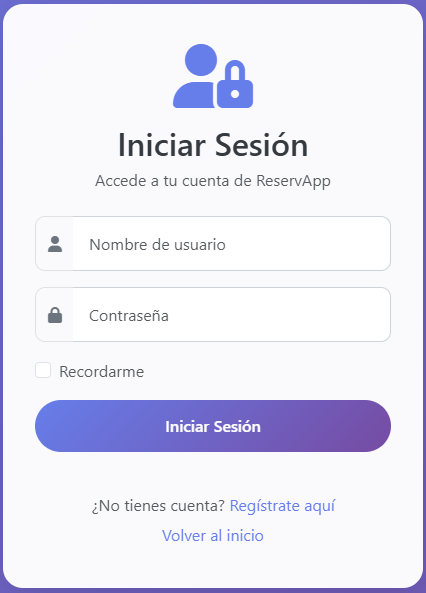
\includegraphics[width=0.5\linewidth]{reservapp_login}
	\caption{Página inicial de la aplicación.}
	\label{fig:reservapp_login}
\end{figure}

\subsubsection{Registro de un nuevo usuario}
Nada más acceder a la aplicación, se mostrará por defecto la página de inicio, tal y como se puede ver en la figura ~\ref{fig:reservapp_login}. Si es la primera vez que se accede a la aplicación, será necesario crear una cuenta para poder acceder a las funcionalidades de reserva. Estos son los pasos a seguir:

\begin{enumerate}
   \item \textbf{Acceder a la página de registro}:

   \begin{itemize}
      \item Desde la página de inicio, hacer clic en ``Regístrate aquí''.
      \item O navegar directamente a ``/registro''.
   \end{itemize}
   \item \textbf{Completar el formulario de registro}:
   \begin{itemize}

      \begin{figure}[H]
         \centering
         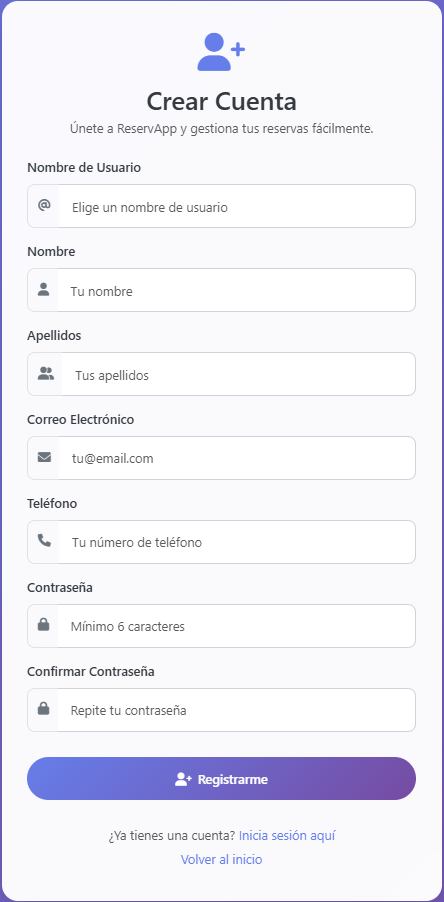
\includegraphics[width=0.5\linewidth]{reservapp_registro}
         \caption{Página para el registro de usuario.}
         \label{fig:reservapp_registro}
      \end{figure}

      \item Al acceder, se mostrará una página como se muestra en la figura ~\ref{fig:reservapp_registro}.
      \item \textbf{Nombre de Usuario (ID de Usuario)}: Introducir un identificador único de 3-10 caracteres alfanuméricos (sin espacios ni símbolos especiales).
      \item \textbf{Nombre}: Introducir el nombre (máximo 50 caracteres).
      \item \textbf{Apellidos}: Introducir los apellidos (máximo 50 caracteres).
      \item \textbf{Correo Electrónico}: Introducir una dirección de email válida y única.
      \item \textbf{Teléfono}: Introducir número de teléfono (5-12 caracteres).
      \item \textbf{Contraseña}: Crear una contraseña segura.
      \item \textbf{Confirmar Contraseña}: Repetir la contraseña para verificación.
   \end{itemize}
   \item \textbf{Enviar el formulario}:
   \begin{itemize}
      \item Hacer clic en ``Registrarse''.
      \item El sistema validará los datos y creará la cuenta.
      \item Se mostrará un mensaje de confirmación.
   \end{itemize}
\end{enumerate}

\textbf{Notas importantes}:
\begin{itemize}
   \item El ID de usuario y el correo electrónico deben ser únicos en el sistema.
   \item Todos los campos son obligatorios.
   \item El sistema \emph{hashea} automáticamente las contraseñas.
\end{itemize}

\subsubsection{Inicio de sesión (login)}
En caso de tener un usuario previamente creado se podrá acceder a la aplicación, a través de la página de inicio, tal y como se muestra en la figura~\ref{fig:reservapp_login}, con las credenciales existentes. Estos son los pasos a seguir:

\begin{enumerate}
   \item \textbf{Acceder a la página de login}:

   \begin{itemize}
      \item Navegar a /login o hacer clic en ``Iniciar Sesión''.
   \end{itemize}
   \item \textbf{Introducir credenciales}:
   \begin{itemize}
      \item \textbf{Usuario}: Introducir el ID de usuario registrado.
      \item \textbf{Contraseña}: Introducir la contraseña correspondiente.
      \item Opcionalmente, marcar ``Recordarme'' para mantener la sesión activa.
   \end{itemize}
   \item \textbf{Iniciar sesión}:
   \begin{itemize}
      \item Hacer clic en ``Iniciar Sesión''.
      \item El sistema redirigirá al menú principal tras la autenticación exitosa.
   \end{itemize}
\end{enumerate}

\textbf{Mensajes de error comunes}:
\begin{itemize}
   \item ``Usuario o contraseña incorrectos'': Verificar las credenciales introducidas.
   \item Usuario bloqueado: Contactar con el administrador del sistema.
\end{itemize}

\subsubsection{Cierre de Sesión}
Pulsando el botón de ``Cerrar Sesión'', provocará el cierre de la sesión actual de forma segura. Estos son los pasos a seguir:

\begin{enumerate}
   \item Desde cualquier página del sistema, hacer clic en el botón ``Cerrar Sesión'' en la sección superior.
   \item El sistema cerrará la sesión y redirigirá a la página de login.
\end{enumerate}

\newpage

\subsection{Navegación Principal}

\subsubsection{Menú Principal}
El menú principal es el centro de control del sistema, organizado en secciones según el rol del usuario.

\begin{figure}[H]
	\centering
		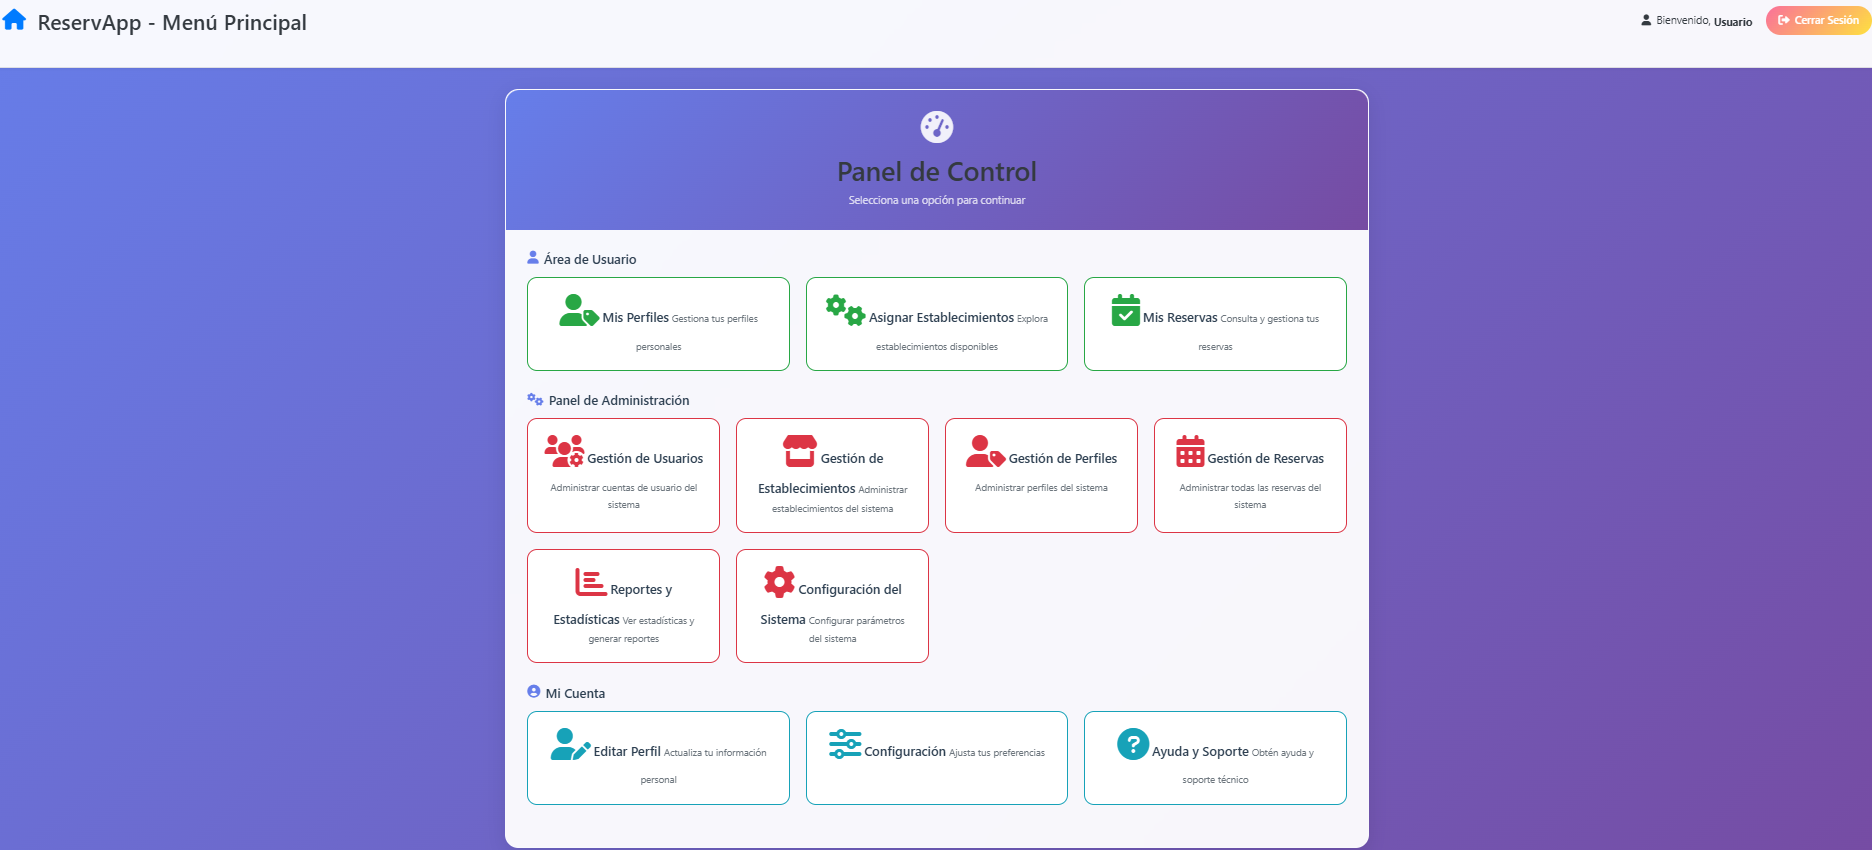
\includegraphics[width=1.0\linewidth]{reservapp_menu_principal_admin}
	\caption{Menú Principal para usuario administrador.}
	\label{fig:reservapp_menu_principal_admin}
\end{figure}

\begin{figure}[H]
	\centering
		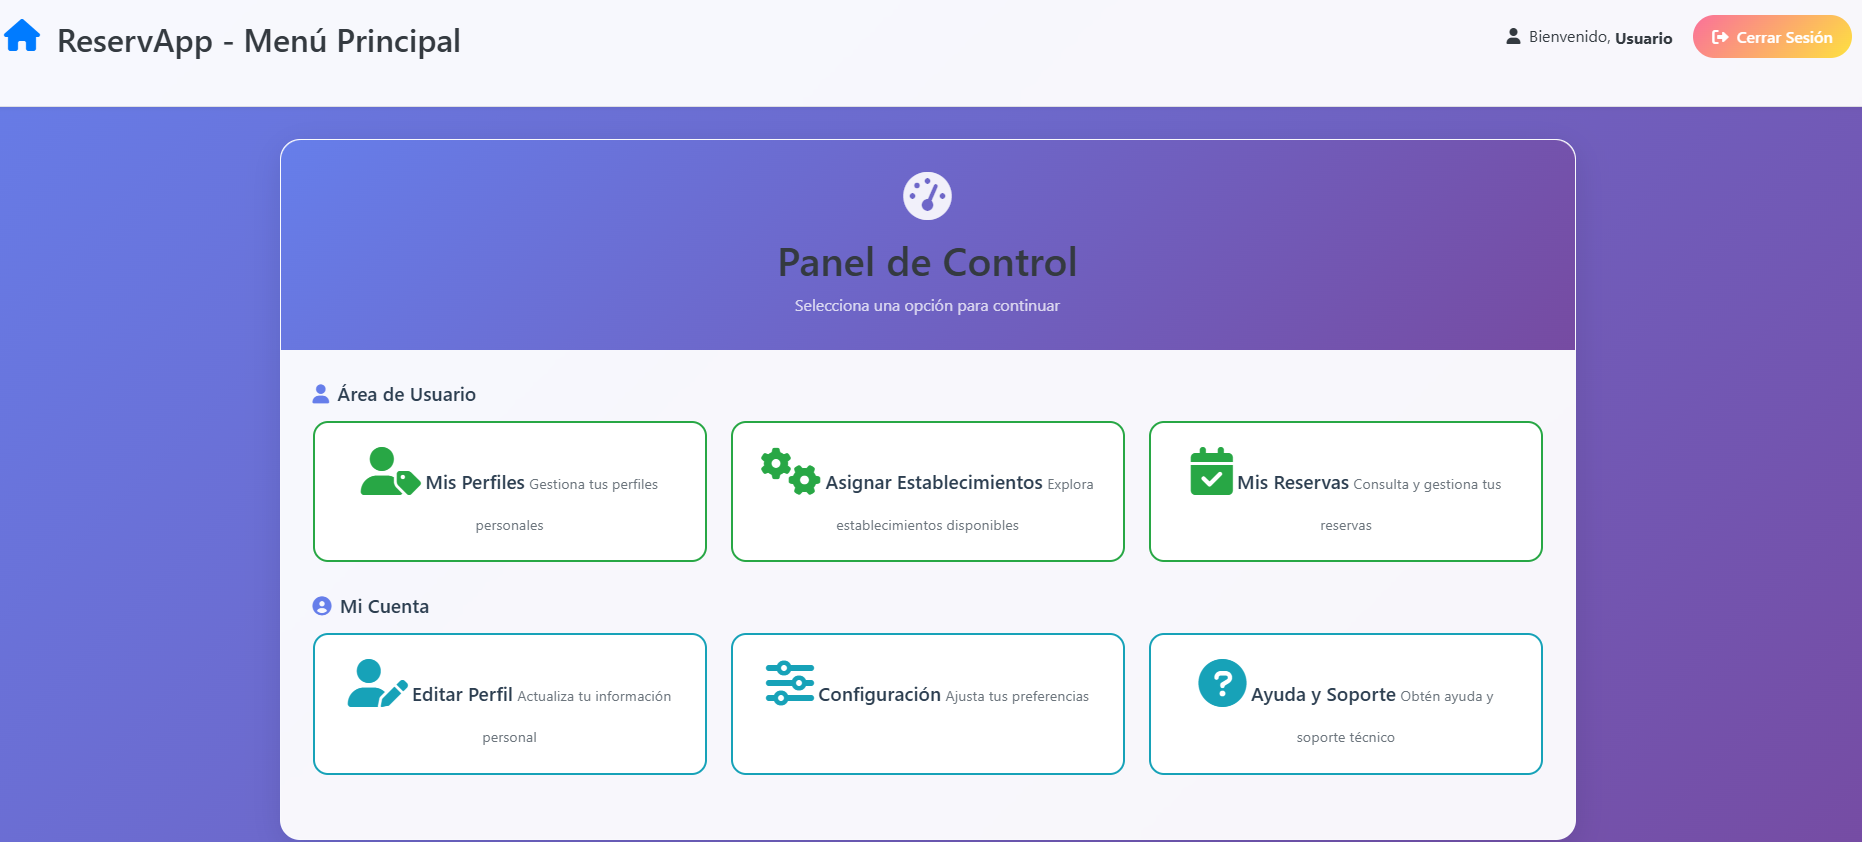
\includegraphics[width=1.0\linewidth]{reservapp_menu_principal_no_admin}
	\caption{Menú Principal para usuario no administrador.}
	\label{fig:reservapp_menu_principal_no_admin}
\end{figure}

\begin{itemize}
   \item Para todos los usuarios, tal y como se muestra en la figura~\ref{fig:reservapp_menu_principal_no_admin}, aparecen disponibles las siguientes secciones:
   \begin{itemize}
      \item \textbf{Área de Usuario}:
      \begin{itemize}
         \item Mis Perfiles: Gestión de perfiles personales.
         \item Asignar Establecimientos: Explorar y solicitar acceso a establecimientos
         \item Mis Reservas: Consultar y gestionar reservas personales
      \end{itemize}
      \item \textbf{Mi Cuenta}:
      \begin{itemize}
         \item Editar Perfil: Actualizar información personal.
         \item Configuración: Ajustar preferencias del usuario.
         \item Ayuda y Soporte: Acceder a documentación y soporte.
      \end{itemize}
   \end{itemize}
   \item Para todos los usuarios que sean administradores, además de las opciones que se muestra para el resto de usuarios,  tal y como se muestra en la figura~\ref{fig:reservapp_menu_principal_admin}, aparecen disponibles las siguientes secciones:
   \begin{itemize}
      \item \textbf{Panel de Administración}:
      \begin{itemize}
         \item Gestión de Usuarios: Administrar cuentas de usuario.
         \item Gestión de Establecimientos: Administrar establecimientos del sistema.
         \item Gestión de Perfiles: Administrar perfiles del sistema.
         \item Gestión de Reservas: Supervisar todas las reservas.
         \item Reportes y Estadísticas: Ver estadísticas del sistema.
         \item Configuración del Sistema: Configurar parámetros globales.
      \end{itemize}
   \end{itemize}
\end{itemize}

\newpage

\subsection{Gestión de Reservas}

\subsubsection{Visualizar Mis Reservas}
Permite consultar los establecimientos disponibles para realizar reservas, tal y como se ilustra en la figura~\ref{fig:reservapp_mis_reservas}. Estos son los pasos a seguir:

\begin{figure}[H]
	\centering
		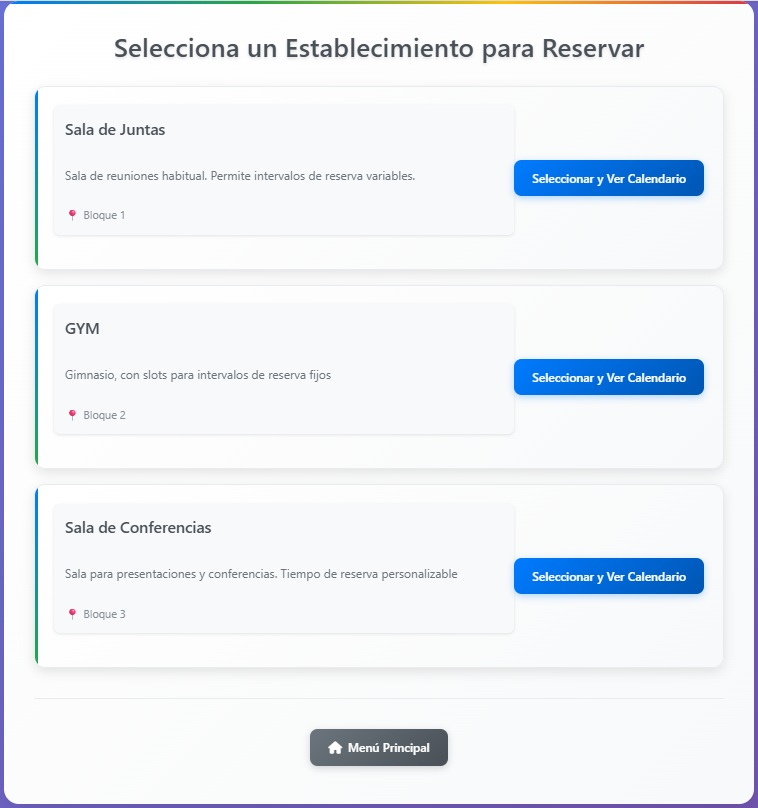
\includegraphics[width=0.75\linewidth]{reservapp_mis_reservas}
	\caption{Página de ``Mis Reservas'' donde se muestran los establecimientos asignados.}
	\label{fig:reservapp_mis_reservas}
\end{figure}

\begin{enumerate}
   \item \textbf{Acceder a ``Mis Reservas''}:
   \begin{itemize}
      \item Desde el menú principal, hacer clic en ``Mis Reservas''.
      \item O navegar directamente a /misreservas.
   \end{itemize}
   \item \textbf{Seleccionar establecimiento}:
   \begin{itemize}
      \item Se mostrará una lista de establecimientos asignados al usuario.
      \item Cada establecimiento muestra:
      \begin{itemize}
         \item Nombre del establecimiento.
         \item Descripción.
         \item Dirección.
      \end{itemize}
      \item Hacer clic en ``Seleccionar y Ver Calendario'' para el establecimiento deseado.
   \end{itemize}
\end{enumerate}

\newpage

\subsubsection{Crear Nueva Reserva}
Permite crear una nueva reserva para un establecimiento en concreto, después de haber seleccionado el establecimiento en la página como la que se ilustra en la figura~\ref{fig:reservapp_mis_reservas}. Estos son los pasos a seguir:

\begin{figure}[H]
	\centering
	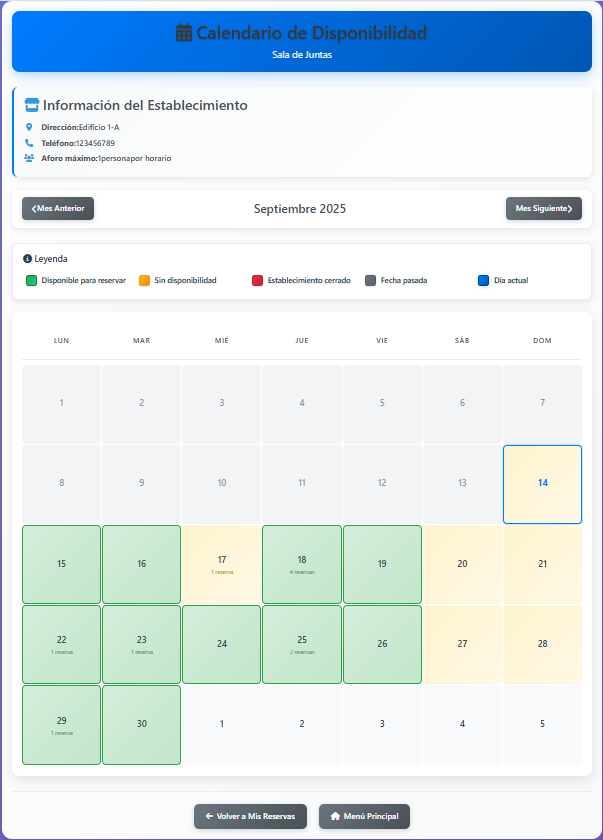
\includegraphics[width=0.85\linewidth]{reservapp_calendario}
	\caption{Página con el calendario del mes actual mostrando la disponibilidad.}
	\label{fig:reservapp_calendario}
\end{figure}

\begin{figure}[H]
	\centering
		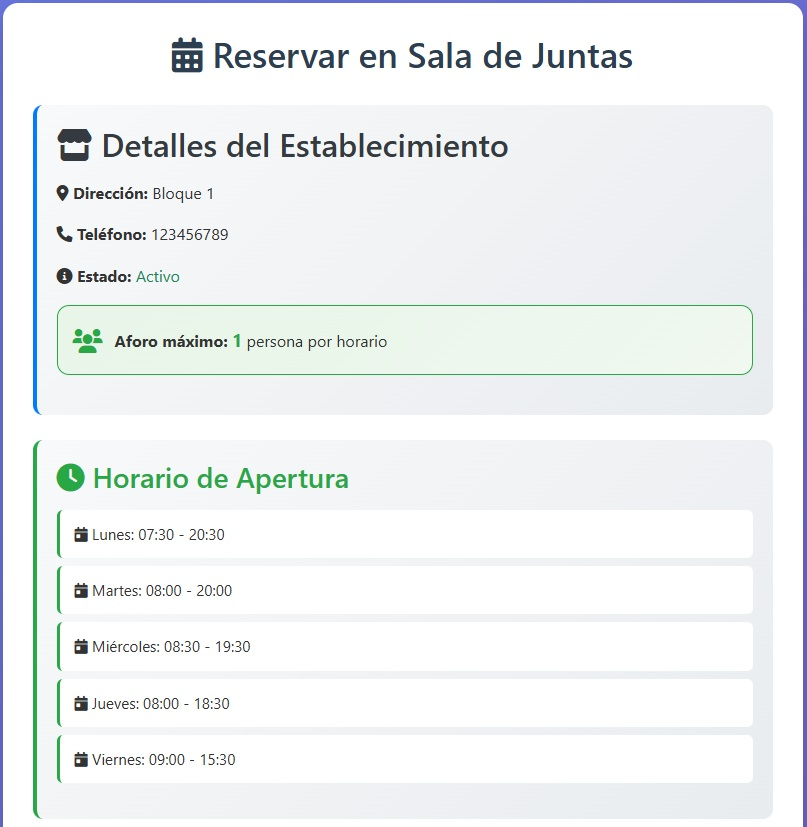
\includegraphics[width=0.5\linewidth]{reservapp_establecimiento_reserva}
	\caption{Página con la información del establecimiento y el régimen horario que tiene.}
	\label{fig:reservapp_establecimiento_reserva}
\end{figure}

\begin{enumerate}
   \item \textbf{Acceder al calendario de reservas}:
   \begin{itemize}
      \item Desde ``Mis Reservas'', seleccionar un establecimiento.
      \item Se muestra un calendario con el mes en curso con la disponibilidad de días para poder concretar una reserva, tal y como se muestra en la figura~\ref{fig:reservapp_calendario}.
   \end{itemize}
   \item \textbf{Seleccionar un día con disponibilidad}:
   \begin{itemize}
      \item Se mostrará la información del establecimiento con su régimen horario, tal y como se muestra en la figura~\ref{fig:reservapp_establecimiento_reserva}.
      \item \textbf{Detalles}: Dirección, teléfono, estado.
      \item \textbf{Aforo}: Número de reservas simultáneas o concurrentes.
      \item \textbf{Horarios de apertura}: Días y horas disponibles para reservas.
   \end{itemize}
   \item \textbf{Seleccionar fecha y hora}:
   \begin{itemize}
      \item \textbf{Fecha}: Seleccionar una fecha futura en el calendario.
      \item \textbf{Horario}: Dependiendo del establecimiento:
      \begin{itemize}
         \item \textbf{Slots predefinidos}: Seleccionar de una lista de horarios disponibles, tal y como se muestra en la figura~\ref{fig:reservapp_reserva_slot}.
         \item \textbf{Horario libre}: Permite escoger entre los periodos variables disponibles, tal y como se muestra en la figura~\ref{fig:reservapp_periodos}, o bien introducir hora de inicio y fin manualmente, tal y como se muestra en la figura~\ref{fig:reservapp_reserva}.
      \end{itemize}
   \end{itemize}

   \begin{figure}[H]
	\centering
		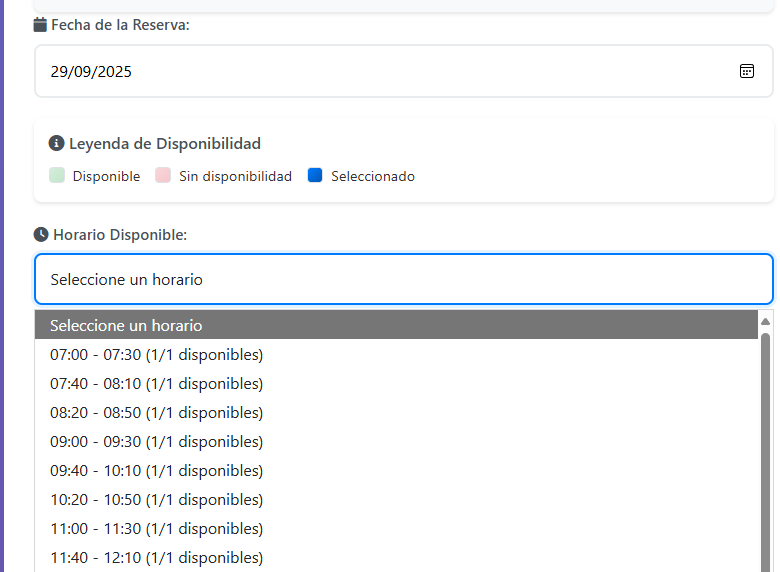
\includegraphics[width=0.5\linewidth]{reservapp_reserva_slot}
	\caption{Sección donde se introducen los datos de la reserva con duración fija.}
	\label{fig:reservapp_reserva_slot}
   \end{figure}

   \begin{figure}[H]
	\centering
	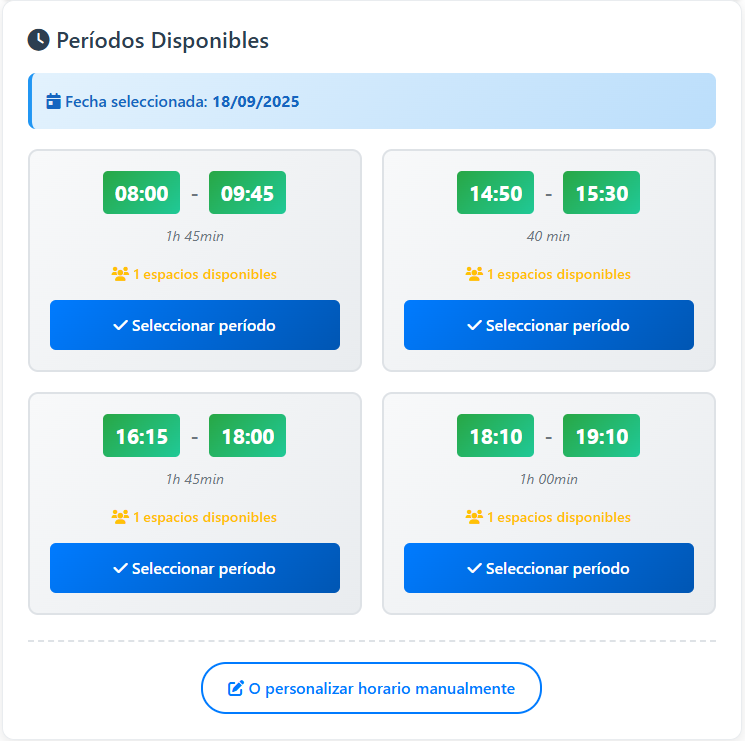
\includegraphics[width=0.5\linewidth]{reservapp_periodos}
	\caption{Sección donde se muestran los periodos variables disponibles.}
	\label{fig:reservapp_periodos}
\end{figure}

   \begin{figure}[H]
	\centering
		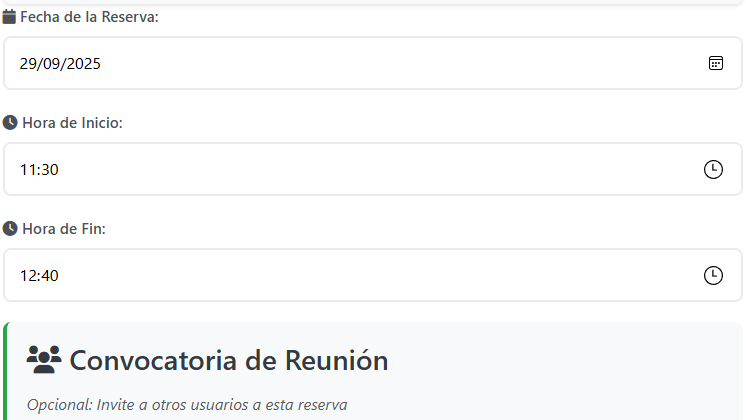
\includegraphics[width=0.5\linewidth]{reservapp_reserva}
	\caption{Sección donde se introducen los datos de la reserva con duración variable.}
	\label{fig:reservapp_reserva}
   \end{figure}

   \item \textbf{Configurar convocatoria (opcional)}:
   \begin{itemize}
      \item \textbf{Enlace de reunión}: Introducir URL de videoconferencia (Google Meet, Zoom, Teams, etc.).
      \item \textbf{Observaciones}: Añadir notas, agenda o temas a tratar.
      \item \textbf{Invitar usuarios}:
      \begin{itemize}
         \item Buscar usuarios por nombre, apellido, ID o email.
         \item Seleccionar usuarios de los resultados de búsqueda.
         \item Los usuarios seleccionados aparecerán en la lista de invitados.
      \end{itemize}
   \end{itemize}
   \item \textbf{Confirmar reserva}:
   \begin{itemize}
      \item Revisar todos los datos introducidos.
      \item Hacer clic en ``Confirmar Reserva''.
      \item El sistema validará la disponibilidad y creará la reserva.
      \item Se enviarán notificaciones por correo al usuario y a los invitados.
   \end{itemize}
\end{enumerate}

\textbf{Validaciones del sistema}:
\begin{itemize}
   \item La fecha debe ser futura.
   \item El horario debe estar dentro de las franjas de apertura del establecimiento.
   \item No debe exceder el aforo máximo del establecimiento.
   \item La hora de fin debe ser posterior a la hora de inicio
\end{itemize}

\subsubsection{Modificar una Reserva}
Permite modificar una reserva previamente creda para un establecimiento en concreto, tal y como se ilustra en la figura~\ref{fig:reservapp_editar_reserva}. Estos son los pasos a seguir:

\begin{figure}[H]
	\centering
		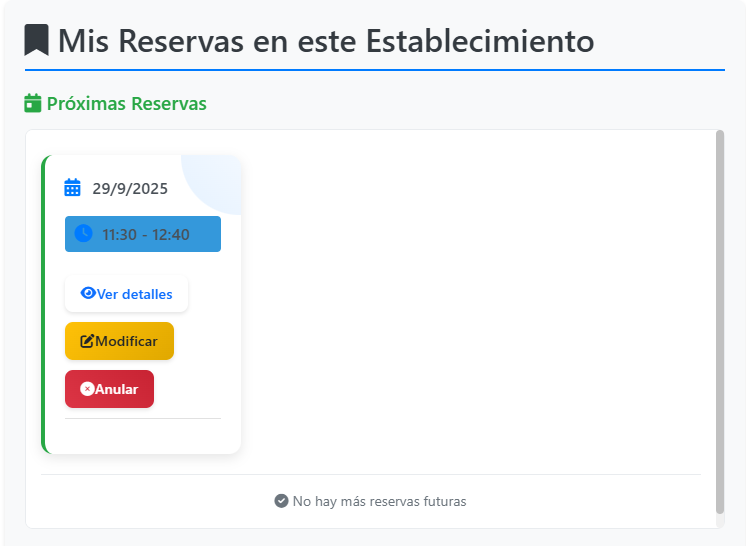
\includegraphics[width=0.5\linewidth]{reservapp_futuras_reservas}
	\caption{Vista del detalle de una reserva futura.}
	\label{fig:reservapp_futuras_reservas}
\end{figure}

\begin{figure}[H]
	\centering
		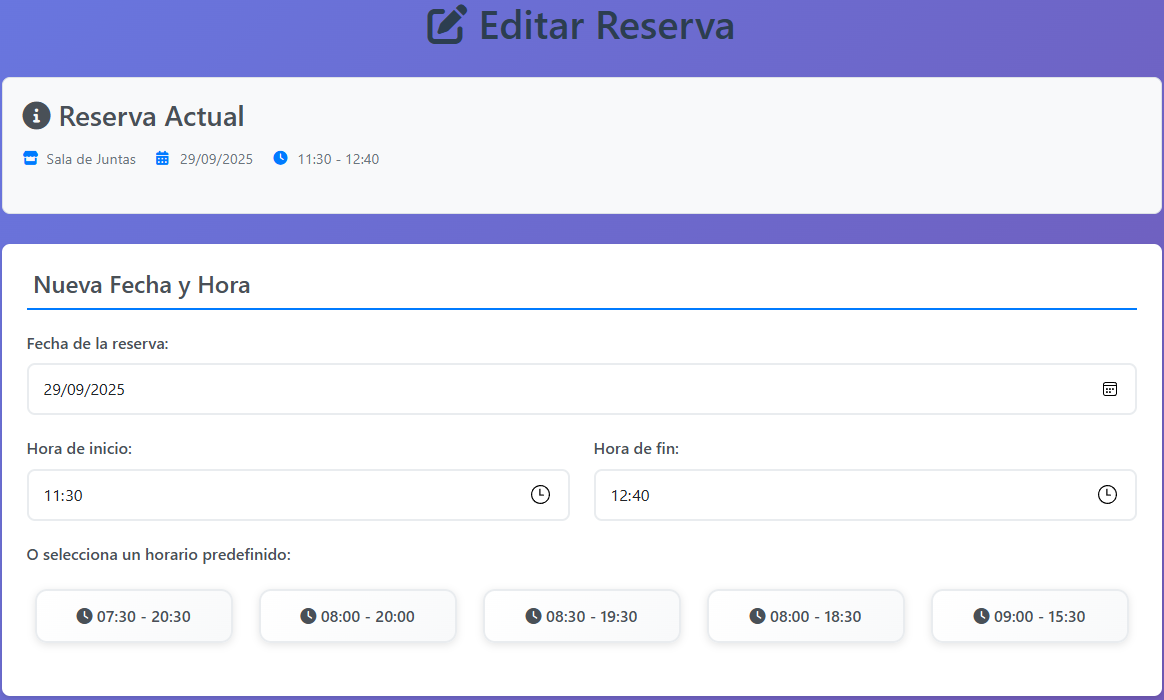
\includegraphics[width=0.5\linewidth]{reservapp_editar_reserva}
	\caption{Página que muestra los datos de la reserva para modificar.}
	\label{fig:reservapp_editar_reserva}
\end{figure}

\begin{enumerate}
   \item \textbf{Localizar la reserva}:
   \begin{itemize}
      \item Desde el calendario del establecimiento, buscar la reserva en ``Próximas Reservas''.
      \item Hacer clic en ``Modificar'' en la reserva deseada. Aparecerá como la imagen de la figura~\ref{fig:reservapp_futuras_reservas}.
   \end{itemize}
   \item \textbf{Editar datos de la reserva}:
   \begin{itemize}
      \item \textbf{Fecha y hora}: Cambiar según disponibilidad.
      \item \textbf{Convocatoria}: Modificar enlace, observaciones o lista de invitados.
      \item Todos los campos son editables siguiendo las mismas reglas que en la creación.
   \end{itemize}
   \item \textbf{Configurar convocatoria (opcional)}:
   \begin{itemize}
      \item \textbf{Enlace de reunión}: Introducir URL de videoconferencia (Google Meet, Zoom, Teams, etc.).
      \item \textbf{Observaciones}: Añadir notas, agenda o temas a tratar.
      \item \textbf{Invitar usuarios}:
      \begin{itemize}
         \item Buscar usuarios por nombre, apellido, ID o email.
         \item Seleccionar usuarios de los resultados de búsqueda.
         \item Los usuarios seleccionados aparecerán en la lista de invitados.
      \end{itemize}
   \end{itemize}
   \item \textbf{Guardar cambios}:
   \begin{itemize}
      \item Hacer clic en ``Guardar Cambios''.
      \item El sistema validará los nuevos datos.
	  \item Se enviarán notificaciones de modificación a todos los involucrados
   \end{itemize}
\end{enumerate}

\textbf{Restricciones}:
\begin{itemize}
   \item Solo se pueden modificar reservas futuras.
   \item Solo el usuario que creó la reserva puede modificarla.
   \item Las modificaciones están sujetas a disponibilidad.
\end{itemize}

\subsubsection{Anular Reserva}
Permite Anular o cancelar una reserva previamente creada para un establecimiento en concreto. Estos son los pasos a seguir:

\begin{enumerate}
   \item \textbf{Localizar la reserva}:
   \begin{itemize}
      \item Desde el calendario del establecimiento, buscar la reserva en ``Próximas Reservas''.
   \end{itemize}
   \item \textbf{Anular reserva}:
   \begin{itemize}
      \item Hacer clic en ``Anular'' en la reserva deseada.
      \item Confirmar la anulación en el diálogo de confirmación.
      \item El sistema eliminará la reserva y enviará notificaciones de cancelación.
   \end{itemize}
\end{enumerate}

\textbf{Restricciones}:
\begin{itemize}
   \item Solo se pueden anular  reservas futuras.
   \item Solo el usuario que creó la reserva puede anularla.
   \item La anulación es irreversible.
\end{itemize}

\subsubsection{Consultar Historial de Reservas}
Permite consultar las reservas pasadas y futuras, tal y como se ilustra en la figura~\ref{fig:reservapp_historial_reservas}. Estas son las funcionalidades disponibles:

\begin{figure}[H]
	\centering
		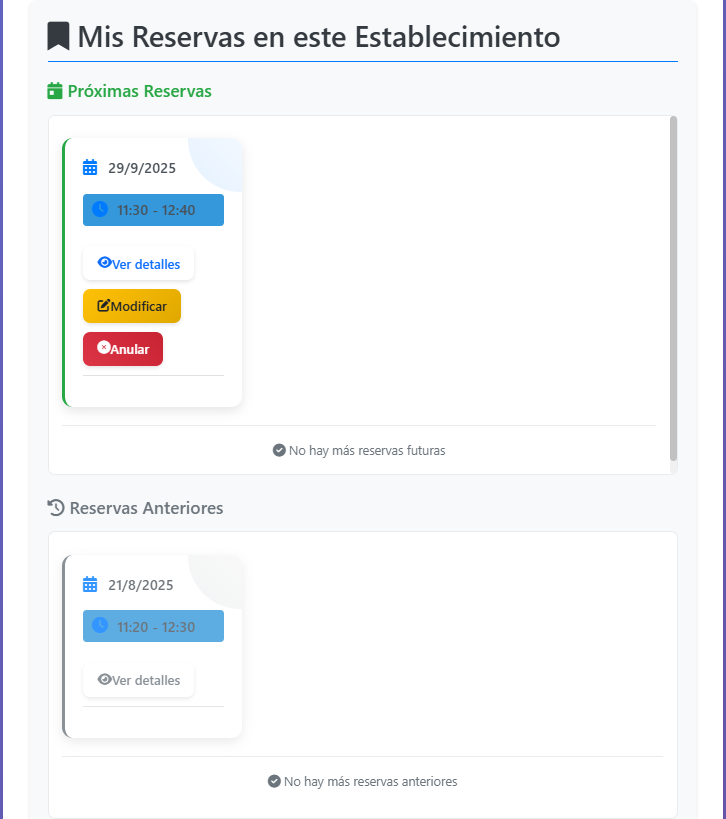
\includegraphics[width=0.5\linewidth]{reservapp_historial_reservas}
	\caption{Página con el historial de reservas.}
	\label{fig:reservapp_historial_reservas}
\end{figure}

\begin{enumerate}
   \item \textbf{Reservas futuras}:
   \begin{itemize}
      \item Lista de próximas reservas ordenadas por fecha.
	  \item Opciones para ver detalles, modificar o anular.
	  \item Información de convocatorias y usuarios invitados.
   \end{itemize}
   \item \textbf{Reservas pasadas}:
   \begin{itemize}
      \item Historial de reservas anteriores.
      \item Solo disponible la opción de ver detalles.
      \item Útil para consultar información de reuniones pasadas.
   \end{itemize}
   \item \textbf{Scroll infinito}:
   \begin{itemize}
      \item Las reservas se cargan dinámicamente al hacer scroll.
      \item Mejora el rendimiento con grandes cantidades de reservas.
   \end{itemize}
\end{enumerate}

\subsection{Gestión de Convocatorias}

\subsubsection{Crear Convocatoria}
Permite invitar a otros usuarios a una reserva y organizar reuniones, tal y como se ilustra en la figura~\ref{fig:reservapp_convocatoria}. Estos son los pasos a seguir:

\begin{figure}[H]
	\centering
		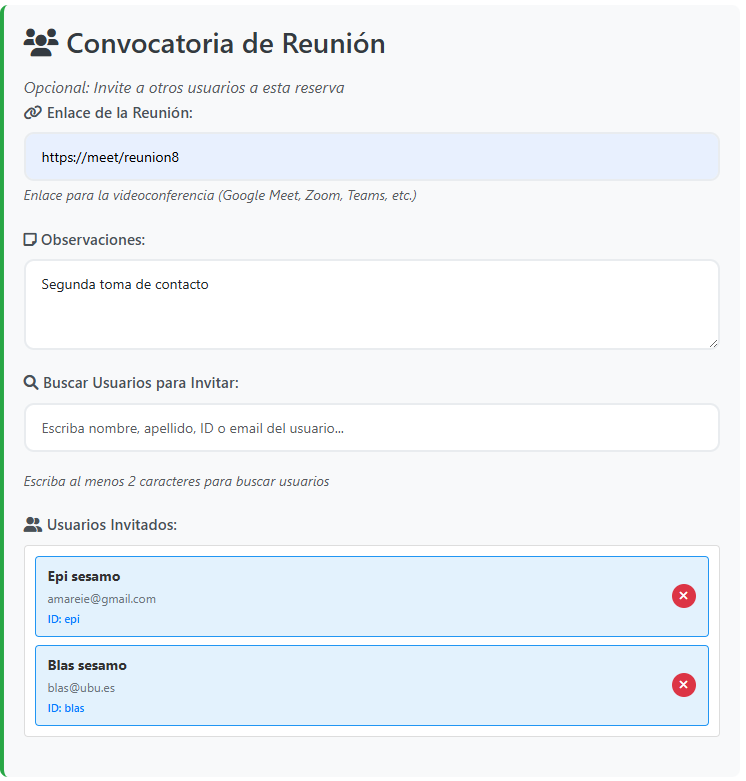
\includegraphics[width=0.5\linewidth]{reservapp_convocatoria}
	\caption{Sección de convocatoria vinculada a la reserva.}
	\label{fig:reservapp_convocatoria}
\end{figure}

\begin{enumerate}
   \item \textbf{Enlace de reunión}:
   \begin{itemize}
      \item URL de plataforma de videoconferencia.
      \item Formatos soportados: Google Meet, Zoom, Microsoft Teams, etc.
	  \item Campo opcional pero recomendado para reuniones virtuales.
   \end{itemize}
   \item \textbf{Observaciones}:
   \begin{itemize}
      \item Agenda de la reunión.
      \item Temas a tratar.
      \item Notas adicionales.
      \item Preparativos necesarios.
   \end{itemize}
   \item \textbf{Lista de invitados}:
   \begin{itemize}
      \item Búsqueda de usuarios por múltiples criterios.
      \item Selección múltiple de participantes.
      \item Vista previa de usuarios seleccionados.
   \end{itemize}
\end{enumerate}

\subsubsection{Gestionar Invitados}
Permite invitar a otros usuarios a una reserva y organizar reuniones, tal y como se ilustra en la figura~\ref{fig:reservapp_convocatoria}. Estos son los pasos a seguir:

\begin{enumerate}
   \item \textbf{Buscar usuarios}:
   \begin{itemize}
      \item Introducir al menos 2 caracteres en el campo de búsqueda.
      \item El sistema buscará por nombre, apellidos, ID de usuario o email.
	  \item Se mostrarán resultados en tiempo real.
   \end{itemize}
   \item \textbf{Seleccionar invitados}:
   \begin{itemize}
      \item Hacer clic en el usuario deseado de los resultados.
      \item El usuario se añadirá a la lista de invitados.
      \item Los usuarios ya seleccionados aparecen deshabilitados en futuras búsquedas.
   \end{itemize}
   \item \textbf{Gestionar lista de invitados}:
   \begin{itemize}
      \item Ver lista completa de usuarios invitados.
      \item Eliminar invitados haciendo clic en el botón ``X''.
      \item La lista se actualiza dinámicamente.
   \end{itemize}
\end{enumerate}

\subsubsection{Notificaciones de Convocatoria}
Permite invitar a otros usuarios a una reserva y organizar reuniones, tal y como se ilustra en la sección inferior de la figura~\ref{fig:reservapp_mis_reservas}. Estos son los pasos a seguir:

\begin{enumerate}
   \item \textbf{Creación de reserva con convocatoria}:
   \begin{itemize}
      \item Se envía email al creador de la reserva.
      \item Se envía email a todos los usuarios invitados.
	  \item Incluye detalles de fecha, hora, lugar y enlace de reunión.
   \end{itemize}
   \item \textbf{Modificación de reserva}:
   \begin{itemize}
      \item Notificación automática a todos los participantes.
      \item Incluye los cambios realizados.
   \end{itemize}
   \item \textbf{Anulación de reserva}:
   \begin{itemize}
      \item Notificación inmediata a todos los involucrados.
      \item Confirmación de cancelación.
   \end{itemize}
\end{enumerate}

\subsection{Gestión de Estbalecimientos}

\subsubsection{Explorar Establecimientos Disponibles}
Visualizar y solicitar acceso a nuevos establecimientos, tal y como se ilustra en la figura~\ref{fig:reservapp_asignacion_establecimiento}. Estos son los pasos a seguir:

\begin{figure}[H]
	\centering
		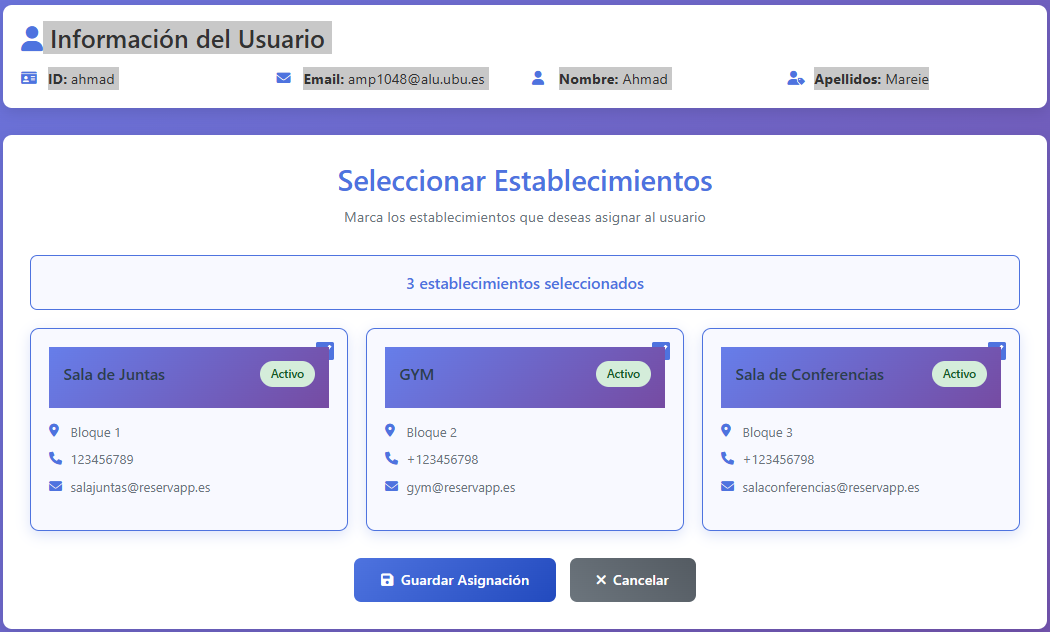
\includegraphics[width=0.5\linewidth]{reservapp_asignacion_establecimiento}
	\caption{Página de Establecimientos disponibles.}
	\label{fig:reservapp_asignacion_establecimiento}
\end{figure}

\begin{enumerate}
   \item \textbf{Acceder a asignación de establecimientos}:
   \begin{itemize}
      \item Desde el menú principal, hacer clic en ``Asignar Establecimientos''.
      \item O navegar a /establecimientos/asignar.
   \end{itemize}
   \item \textbf{Revisar establecimientos disponibles}:
   \begin{itemize}
      \item Lista completa de establecimientos del sistema.
      \item Información detallada de cada establecimiento.
	  \begin{itemize}
         \item Nombre y descripción.
         \item Tipo de establecimiento.
		 \item Capacidad y aforo.
		 \item Horarios de funcionamiento.
		 \item Información de contacto.
      \end{itemize}
   \end{itemize}
   \item \textbf{Solicitar asignación}:
   \begin{itemize}
      \item Seleccionar los establecimientos deseados mediante checkboxes.
      \item Hacer clic en ``Guardar Asignación''.
      \item El sistema procesará la solicitud.
   \end{itemize}
\end{enumerate}

\textbf{Nota}: La asignación puede requerir aprobación administrativa según la configuración del sistema.


\subsubsection{Gestionar Establecimientos Asignados}
Visualizar y solicitar acceso a nuevos establecimientos, tal y como se ilustra en la figura~\ref{fig:reservapp_asignacion_establecimiento}. Estos son los pasos a seguir:

\begin{enumerate}
   \item \textbf{Funcionalidades disponibles}:
   \begin{itemize}
      \item \textbf{Ver establecimientos asignados}.
      \begin{itemize}
         \item Lista de establecimientos a los que el usuario tiene acceso.
         \item Estado de cada establecimiento (activo/inactivo).
      \end{itemize}

      \item \textbf{Acceder a calendarios de reserva}.
      \begin{itemize}
         \item Hacer clic en cualquier establecimiento asignado.
         \item Acceso directo al sistema de reservas del establecimiento.
      \end{itemize}
   \end{itemize}
\end{enumerate}

\subsection{Gestión de Perfil Personal}

\subsubsection{Editar Información Personal}
Permite actualizar los datos personales del usuario, tal y como se ilustra en la figura~\ref{fig:reservapp_editar_perfil}. Estos son los pasos a seguir:

\begin{figure}[H]
	\centering
		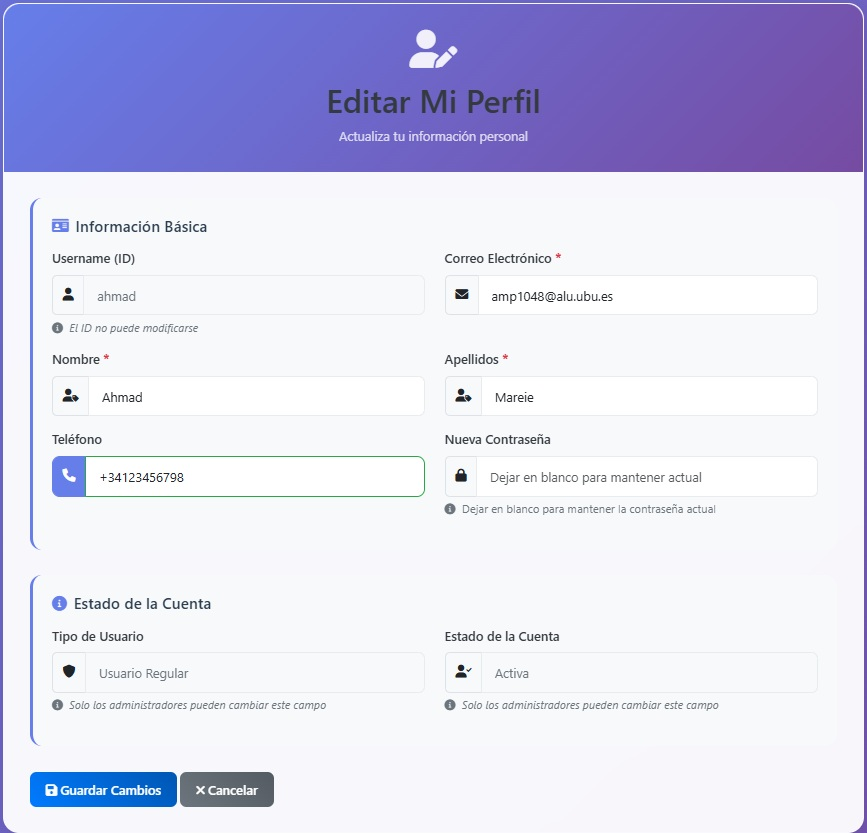
\includegraphics[width=0.5\linewidth]{reservapp_editar_perfil}
	\caption{Página de edición del perfil del usuario.}
	\label{fig:reservapp_editar_perfil}
\end{figure}

\begin{enumerate}
   \item \textbf{Acceder a edición de perfil}:
   \begin{itemize}
      \item Desde el menú principal, hacer clic en ``Editar Perfil''.
      \item O navegar a /perfiles.
   \end{itemize}
   \item \textbf{Modificar información}:
   \begin{itemize}
      \item \textbf{Datos personales}: Nombre, apellidos, teléfono.
      \item \textbf{Correo electrónico}: Cambiar email (debe ser único).
	  \item \textbf{Contraseña}: Actualizar contraseña (opcional).
   \end{itemize}
   \item \textbf{Guardar cambios}:
   \begin{itemize}
      \item Hacer clic en ``Guardar Cambios''.
      \item El sistema validará los datos y aplicará las modificaciones.
   \end{itemize}
\end{enumerate}

\textbf{Restricciones}:
\begin{itemize}
   \item El ID de usuario no se puede modificar.
   \item El correo electrónico debe ser único en el sistema.
   \item Los cambios de contraseña requieren confirmación.
\end{itemize}

\subsection{Funcionalidades Administrativas}
Nota: Las siguientes funcionalidades están disponibles únicamente para usuarios con rol de administrador.

\subsubsection{Gestión de Usuarios: Visualizar Usuarios}
Permite administrar todas las cuentas de usuario del sistema, tal y como se ilustra en la figura~\ref{fig:reservapp_gestion_usuarios}. Estos son los pasos a seguir:

\begin{figure}[H]
	\centering
		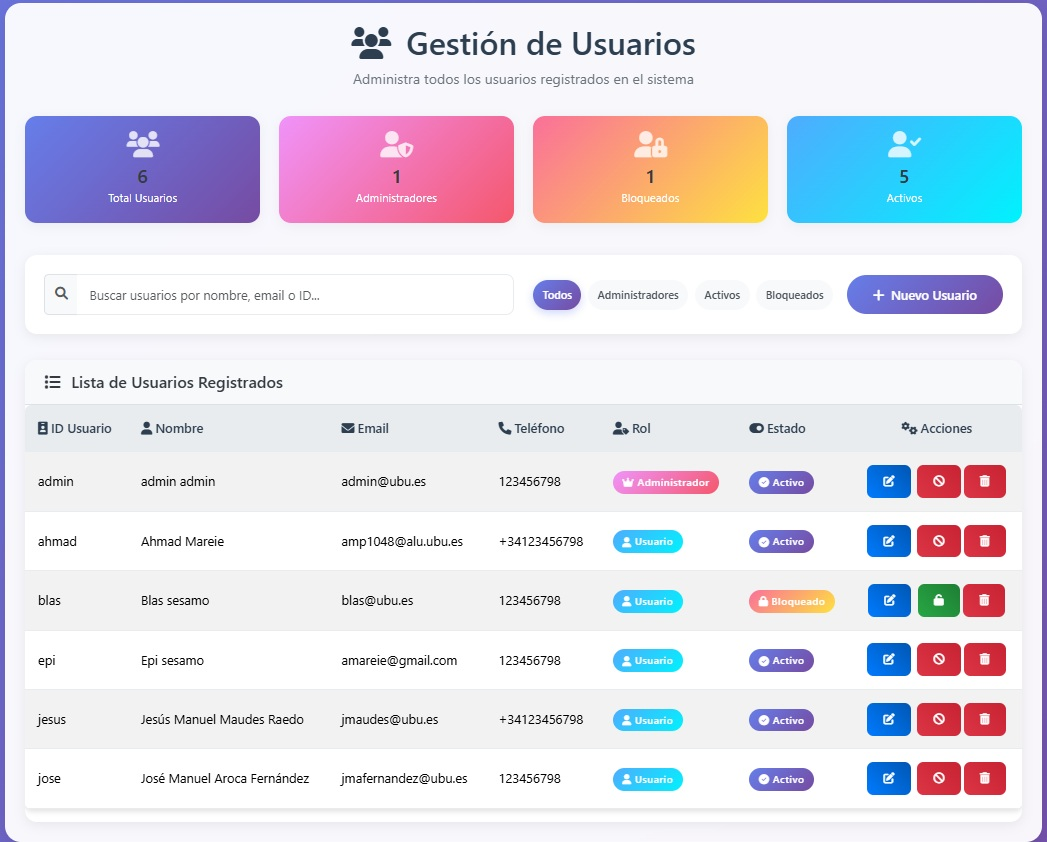
\includegraphics[width=0.5\linewidth]{reservapp_gestion_usuarios}
	\caption{Página de gestión de usuarios.}
	\label{fig:reservapp_gestion_usuarios}
\end{figure}

\begin{enumerate}
   \item \textbf{Acceder a gestión de usuarios}:
   \begin{itemize}
      \item Desde el menú principal, hacer clic en ``Gestión de Usuarios''.
      \item O navegar a /admin/usuarios.
   \end{itemize}
   \item \textbf{Revisar estadísticas del sistema}:
   \begin{itemize}
      \item \textbf{Total de usuarios}: Número total de cuentas registradas.
      \item \textbf{Administradores}: Cantidad de usuarios con privilegios administrativos.
	  \item \textbf{Usuarios bloqueados}: Cuentas deshabilitadas.
	  \item \textbf{Usuarios activos}: Cuentas habilitadas y funcionales.
   \end{itemize}
   \item \textbf{Utilizar herramientas de búsqueda y filtrado}:
   \begin{itemize}
      \item \textbf{Búsqueda}: Buscar por nombre, email o ID de usuario.
	  \item \textbf{Filtros}: Mostrar todos, solo administradores, solo activos, solo bloqueados.
      \item Los resultados se actualizan en tiempo real.
   \end{itemize}
\end{enumerate}

\subsubsection{Gestión de Usuarios: Crear nuevo usuario}
Permite crear un nuevo usuario en el sistema, tal y como se ilustra en la figura~\ref{fig:reservapp_nuevo_usuario}. Estos son los pasos a seguir:

\begin{figure}[H]
	\centering
		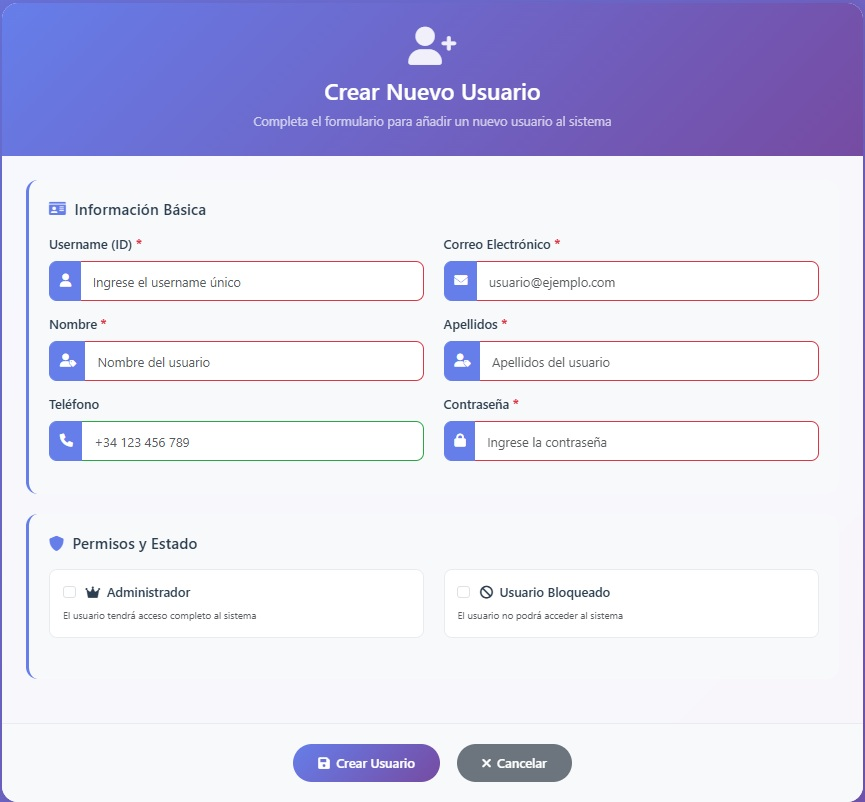
\includegraphics[width=0.5\linewidth]{reservapp_nuevo_usuario}
	\caption{Página con la ficha de usuario.}
	\label{fig:reservapp_nuevo_usuario}
\end{figure}

\begin{enumerate}
   \item \textbf{Iniciar creación}:
   \begin{itemize}
      \item Hacer clic en ``Nuevo Usuario''.
      \item Se abrirá el formulario de creación.
   \end{itemize}
   \item \textbf{Completar información del usuario}:
   \begin{itemize}
      \item \textbf{ID de Usuario}: Identificador único (3-10 caracteres alfanuméricos).
      \item \textbf{Datos personales}: Nombre, apellidos, teléfono.
	  \item \textbf{Correo electrónico}: Email único del usuario.
	  \item \textbf{Contraseña}: Contraseña inicial (obligatoria para nuevos usuarios).
	  \item \textbf{Rol}: Seleccionar si será administrador o usuario regular.
	  \item \textbf{Estado}: Definir si la cuenta estará activa o bloqueada.
   \end{itemize}
   \item \textbf{Guardar usuario}:
   \begin{itemize}
      \item Hacer clic en ``Guardar Usuario''.
	  \item El sistema validará los datos y creará la cuenta.
   \end{itemize}
\end{enumerate}

\subsubsection{Gestión de Usuarios: Editar usuario existente}
Permite modificar un usuario existente en el sistema, tal y como se ilustra en la figura~\ref{fig:reservapp_nuevo_usuario}. Estos son los pasos a seguir:

\begin{enumerate}
   \item \textbf{Seleccionar usuario}:
   \begin{itemize}
      \item Desde la lista de usuarios, hacer clic en el botón "Editar" (icono de lápiz).
   \end{itemize}
   \item \textbf{Modificar información}:
   \begin{itemize}
      \item \textbf{Datos personales}: Actualizar nombre, apellidos, teléfono.
      \item \textbf{Correo electrónico}: Cambiar email (debe seguir siendo único).
	  \item \textbf{Contraseña}: Dejar vacío para mantener la actual, o introducir nueva contraseña.
	  \item \textbf{Rol}: Cambiar entre usuario regular y administrador.
	  \item \textbf{Estado}: Modificar estado de bloqueo.
   \end{itemize}
   \item \textbf{Guardar usuario}:
   \begin{itemize}
      \item Hacer clic en ``Guardar Usuario''.
	  \item Los cambios se aplicarán inmediatamente.
   \end{itemize}
\end{enumerate}

\subsubsection{Gestión de Usuarios: Actualizar el Estado de Usuario}
Permite modificar el estado de un usuario existente en el sistema, tal y como se ilustra en la figura~\ref{fig:reservapp_nuevo_usuario}. Estos son los pasos a seguir:

\begin{enumerate}
   \item \textbf{Bloquear usuario}:
   \begin{enumerate}
      \item Hacer clic en el botón ``Bloquear'' (icono de prohibición) junto al usuario.
	  \item Confirmar la acción en el diálogo de confirmación.
	  \item El usuario no podrá acceder al sistema hasta ser desbloqueado
   \end{enumerate}
   \item \textbf{Desbloquear usuario}:
   \begin{enumerate}
      \item Hacer clic en el botón "Desbloquear" (icono de candado abierto) junto al usuario bloqueado.
      \item Confirmar la acción.
	  \item El usuario recuperará el acceso al sistema.
   \end{enumerate}
   \item \textbf{Eliminar usuario}:
   \begin{enumerate}
      \item Hacer clic en el botón "Eliminar" (icono de papelera) junto al usuario.
	  \item Confirmar la eliminación (acción irreversible).
	  \item Se eliminará la cuenta y todos sus datos asociados
   \end{enumerate}
\end{enumerate}

\textbf{Restricciones}:
\begin{itemize}
   \item Los administradores no pueden eliminar su propia cuenta.
   \item La eliminación de usuarios es irreversible.
   \item Se recomienda bloquear antes que eliminar para preservar el historial.
\end{itemize}

\subsubsection{Gestión de Establecimientos: Visualizar Establecimientos}
Permite administrar todos los establecimientos del sistema, tal y como se ilustra en la figura~\ref{fig:reservapp_gestion_establecimientos}. Estos son los pasos a seguir:

\begin{figure}[H]
	\centering
		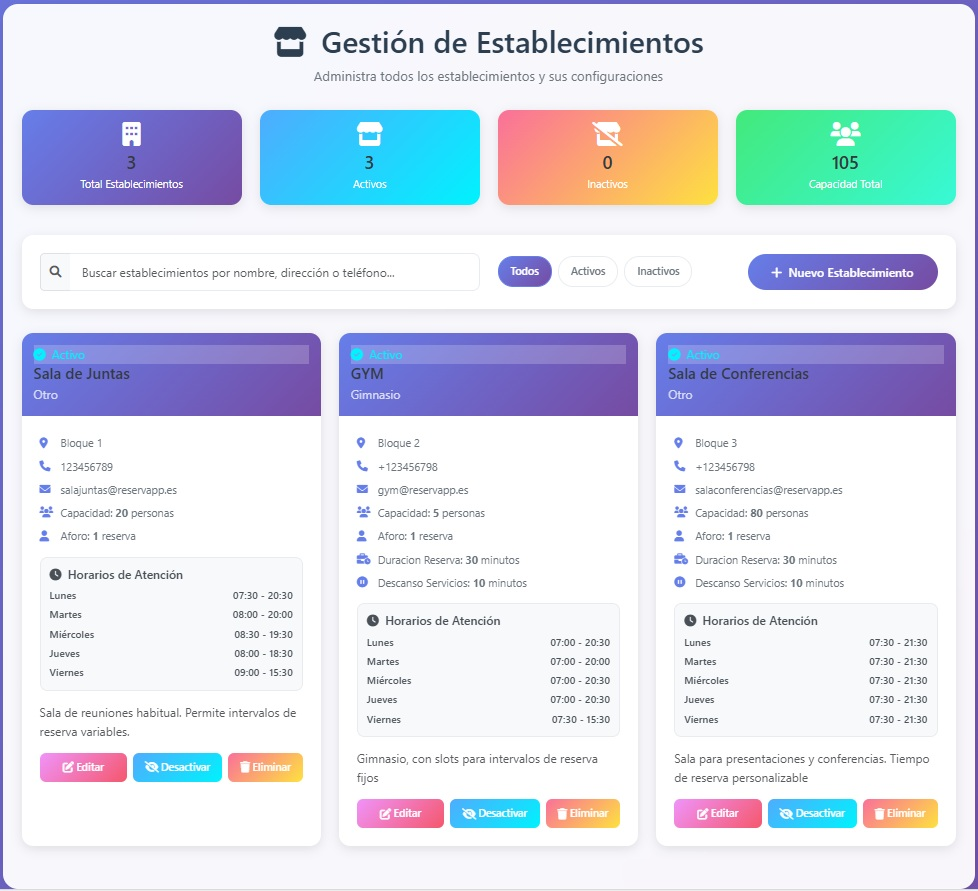
\includegraphics[width=0.5\linewidth]{reservapp_gestion_establecimientos}
	\caption{Página de Gestión de Establecimientos.}
	\label{fig:reservapp_gestion_establecimientos}
\end{figure}

\begin{enumerate}
   \item \textbf{Acceder a gestión de establecimientos}:
   \begin{itemize}
      \item Desde el menú principal, hacer clic en ``Gestión de Establecimientos''.
      \item O navegar a /admin/establecimientos.
   \end{itemize}
   \item \textbf{Revisar estadísticas}:
   \begin{itemize}
      \item \textbf{Total de establecimientos}: Número total registrado.
      \item \textbf{Establecimientos activos}: Disponibles para reservas.
	  \item \textbf{Establecimientos inactivos}: Temporalmente deshabilitados.
	  \item \textbf{Capacidad total}: Suma de capacidades de todos los establecimientos.
   \end{itemize}
   \item \textbf{Utilizar herramientas de búsqueda}:
   \begin{itemize}
      \item \textbf{Búsqueda}: Buscar por nombre, dirección o teléfono.
	  \item \textbf{Filtros}: Mostrar todos, solo activos, solo inactivos.
   \end{itemize}
\end{enumerate}

\subsubsection{Gestión de Establecimientos: Crear Nuevo Establecimiento}
Permite crear un nuevo establecimiento en el sistema, tal y como se ilustra en la figura~\ref{fig:reservapp_nuevo_establecimientos}. Estos son los pasos a seguir:

\begin{figure}[H]
	\centering
		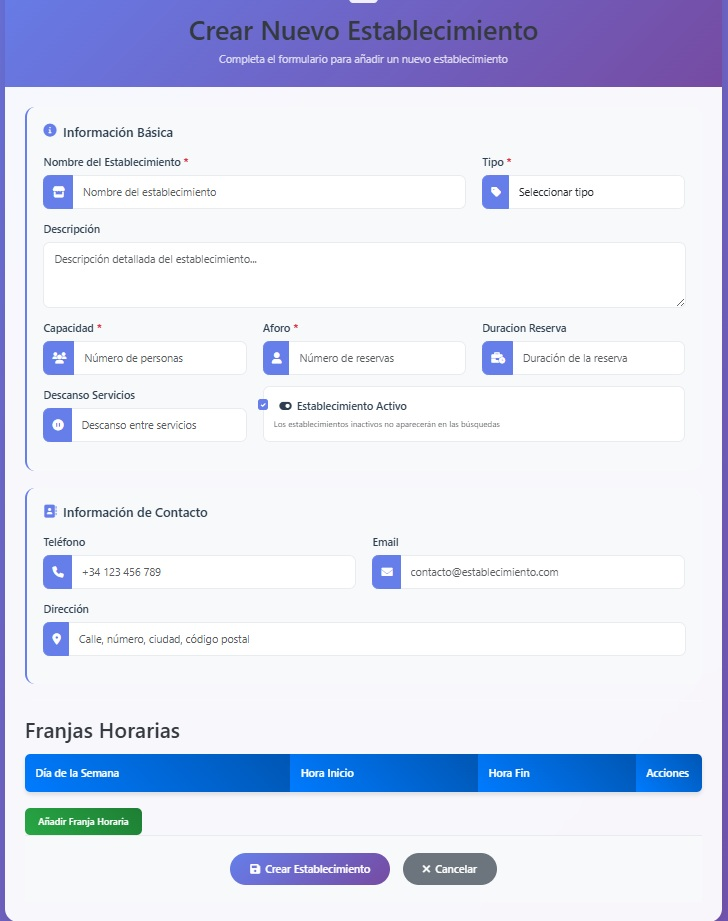
\includegraphics[width=0.5\linewidth]{reservapp_nuevo_establecimientos}
	\caption{Página de Nuevo Establecimiento.}
	\label{fig:reservapp_nuevo_establecimientos}
\end{figure}

\begin{enumerate}
   \item \textbf{Iniciar creación}:
   \begin{itemize}
      \item Hacer clic en ``Nuevo Establecimiento''.
   \end{itemize}
   \item \textbf{Completar información básica}:
   \begin{itemize}
      \item \textbf{Nombre}: Denominación del establecimiento (máximo 80 caracteres).
      \item \textbf{Descripción}: Descripción detallada (máximo 250 caracteres).
	  \item \textbf{Tipo}: Categoría del establecimiento.
	  \item \textbf{Dirección}: Ubicación física.
	  \item \textbf{Teléfono}: Número de contacto.
	  \item \textbf{Email}: Correo electrónico de contacto.
   \end{itemize}
   \item \textbf{Configurar parámetros operativos}:
   \begin{itemize}
      \item \textbf{Búsqueda}: Buscar por nombre, dirección o teléfono.
	  \item \textbf{Filtros}: Mostrar todos, solo activos, solo inactivos.
   \end{itemize}
   \item \textbf{Definir horarios de funcionamiento}:
   \begin{itemize}
      \item \textbf{Búsqueda}: Buscar por nombre, dirección o teléfono.
	  \item \textbf{Filtros}: Mostrar todos, solo activos, solo inactivos.
   \end{itemize}
   \item \textbf{Guardar establecimiento}:
   \begin{itemize}
      \item Hacer clic en ``Guardar Establecimiento''.
	  \item El establecimiento se creará en estado activo por defecto.
   \end{itemize}
\end{enumerate}

\subsubsection{Gestión de Establecimientos: Editar Establecimiento Existente}
Permite editar un establecimiento previamente creado en el sistema, tal y como se ilustra en la figura~\ref{fig:reservapp_nuevo_establecimientos}. Estos son los pasos a seguir:

\begin{enumerate}
   \item \textbf{Seleccionar establecimiento}:
   \begin{itemize}
      \item Hacer clic en ``Editar'' en la tarjeta del establecimiento deseado.
   \end{itemize}
   \item \textbf{Modificar información}:
   \begin{itemize}
      \item Actualizar cualquier campo de información básica.
      \item Ajustar parámetros operativos según necesidades.
	  \item Modificar horarios de funcionamiento.
   \end{itemize}
   \item \textbf{Guardar cambios}:
   \begin{itemize}
      \item Hacer clic en ``Guardar Cambios''.
	  \item Los cambios se aplicarán inmediatamente.
   \end{itemize}
\end{enumerate}

\subsubsection{Gestión de Establecimientos: Actualizar Estado de Establecimientos}
Permite actualizar el estado de un establecimiento previamente creado en el sistema, tal y como se ilustra en la figura~\ref{fig:reservapp_gestion_establecimientos}. Estos son los pasos a seguir:

\begin{itemize}
   \item \textbf{Activar/Desactivar establecimiento}:
   \begin{enumerate}
      \item Hacer clic en ``Activar'' o ``Desactivar'' según el estado actual.
	  \item Confirmar la acción
	  \item Los establecimientos inactivos no estarán disponibles para nuevas reservas
   \end{enumerate}
   \item \textbf{Eliminar establecimiento}:
   \begin{enumerate}
      \item Hacer clic en ``Eliminar''.
      \item Confirmar la eliminación (acción irreversible).
	  \item Se eliminará el establecimiento y todas sus reservas asociadas.
   \end{enumerate}
\end{itemize}

\subsubsection{Gestión de Perfiles: Visualizar Establecimientos}
Permite administrar todos los perfiles del sistema, tal y como se ilustra en la figura~\ref{fig:reservapp_gestion_perfiles}. Estos son los pasos a seguir:

\begin{figure}[H]
	\centering
		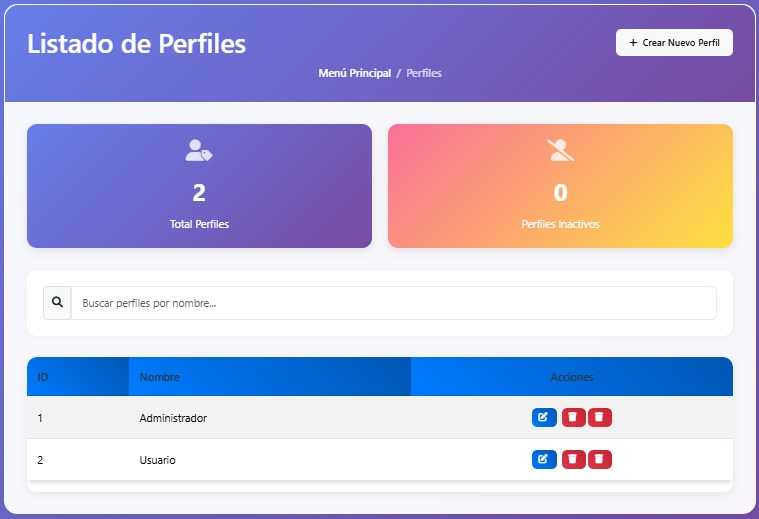
\includegraphics[width=0.5\linewidth]{reservapp_gestion_perfiles}
	\caption{Página de Gestión de Perfiles.}
	\label{fig:reservapp_gestion_perfiles}
\end{figure}

\begin{enumerate}
   \item \textbf{Acceder a gestión de perfiles}:
   \begin{itemize}
      \item Desde el menú principal, hacer clic en ``Gestión de Perfiles''.
      \item O navegar a /admin/perfiles.
   \end{itemize}
   \item \textbf{Revisar perfiles existentes}:
   \begin{itemize}
      \item Lista de todos los perfiles configurados.
      \item Información de cada perfil y sus características.
   \end{itemize}
\end{enumerate}

\subsubsection{Gestión de Perfiles: Crear Nuevo Perfil}
Permite crear un nuevo perfil en el sistema, tal y como se ilustra en la figura~\ref{fig:reservapp_nuevo_perfil}. Estos son los pasos a seguir:

\begin{figure}[H]
	\centering
		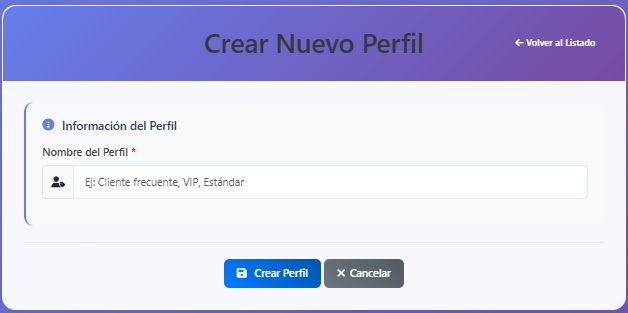
\includegraphics[width=0.5\linewidth]{reservapp_nuevo_perfil}
	\caption{Página de Nuevo Perfil.}
	\label{fig:reservapp_nuevo_perfil}
\end{figure}

\begin{enumerate}
   \item \textbf{Iniciar creación}:
   \begin{itemize}
      \item Hacer clic en ``Nuevo Perfil''.
   \end{itemize}
   \item \textbf{Completar información básica}:
   \begin{itemize}
      \item \textbf{Nombre}: Denominación del perfil.
      \item \textbf{Descripción}: Descripción de las funcionalidades del perfil.
   \end{itemize}
   \item \textbf{Guardar perfil}:
   \begin{itemize}
      \item Hacer clic en ``Guardar Perfil''.
   \end{itemize}
\end{enumerate}

\subsubsection{Gestión de Perfiles: Editar o eliminar Perfiles}
Permite crear un nuevo perfil en el sistema, tal y como se ilustra en la figura~\ref{fig:reservapp_gestion_perfiles}. Estos son los pasos a seguir:

\begin{itemize}
   \item \textbf{Editar perfil}:
   \begin{enumerate}
      \item Hacer clic en ``Editar'' junto al perfil deseado.
	  \item Modificar la información necesaria.
	  \item Guardar los cambios.
   \end{enumerate}
   \item \textbf{Eliminar perfil}:
   \begin{enumerate}
      \item Hacer clic en ``Eliminar'' junto al perfil.
      \item Confirmar la eliminación.
   \end{enumerate}
\end{itemize}

\subsubsection{Supervisión de Reservas: Vista General de Reservas}
Permite monitorear y gestionar todas las reservas del sistema., tal y como se ilustra en la figura~\ref{fig:reservapp_gestion_reservas}. Estos son los pasos a seguir:

\begin{figure}[H]
	\centering
		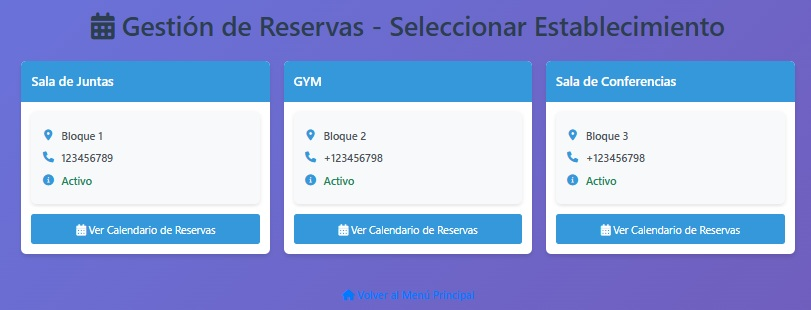
\includegraphics[width=0.5\linewidth]{reservapp_gestion_reservas}
	\caption{Vista previa de los establecimientos para ver las reservas.}
	\label{fig:reservapp_gestion_reservas}
\end{figure}

\begin{enumerate}
   \item \textbf{Acceder a gestión de reservas}:
   \begin{itemize}
      \item Desde el menú principal, hacer clic en ``Gestión de Reservas''.
      \item O navegar a /admin/reservas.
   \end{itemize}
   \item \textbf{Seleccionar establecimiento}:
   \begin{itemize}
      \item Elegir el establecimiento a supervisar de la lista disponible.
   \end{itemize}
\end{enumerate}

\subsubsection{Supervisión de Reservas: Calendario Mensual de Reservas}
Permite ver el calendario mensual de las reservas que tiene un establecimiento, tal y como se ilustra en la figura~\ref{fig:reservapp_calendario_reservas}. Estos son los pasos a seguir:

\begin{figure}[H]
	\centering
		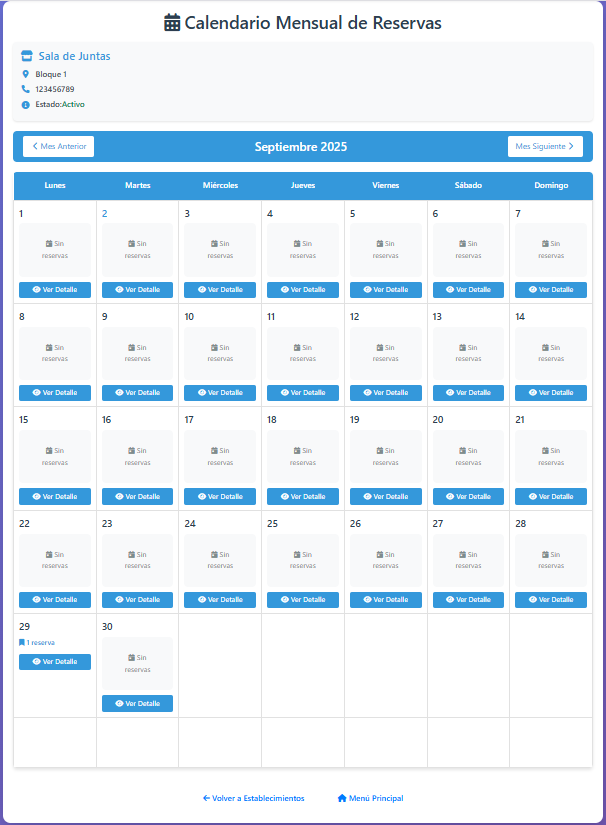
\includegraphics[width=0.5\linewidth]{reservapp_calendario_reservas}
	\caption{Calendario mensual de reservas de un establecimiento.}
	\label{fig:reservapp_calendario_reservas}
\end{figure}

\begin{enumerate}
   \item \textbf{Navegación temporal}:
   \begin{itemize}
      \item Cambiar entre meses y años usando los controles de navegación.
	  \item Vista de calendario mensual con todas las reservas.
   \end{itemize}
   \item \textbf{Información por día}:
   \begin{itemize}
      \item Cada día muestra el número de reservas programadas.
      \item Colores diferentes indican la densidad de reservas.
   \end{itemize}
   \item \textbf{Acceso a detalles diarios}:
   \begin{itemize}
      \item Hacer clic en cualquier día para ver las reservas específicas.
	  \item Vista detallada de todas las reservas del día seleccionado
   \end{itemize}
\end{enumerate}

\subsubsection{Supervisión de Reservas: Detalle de Reservas Diarias}
Permite ver el detalle de una reserva en concreto, tal y como se ilustra en la figura~\ref{fig:reservapp_detalle_reservas}. Estos son los pasos a seguir:

\begin{figure}[H]
	\centering
		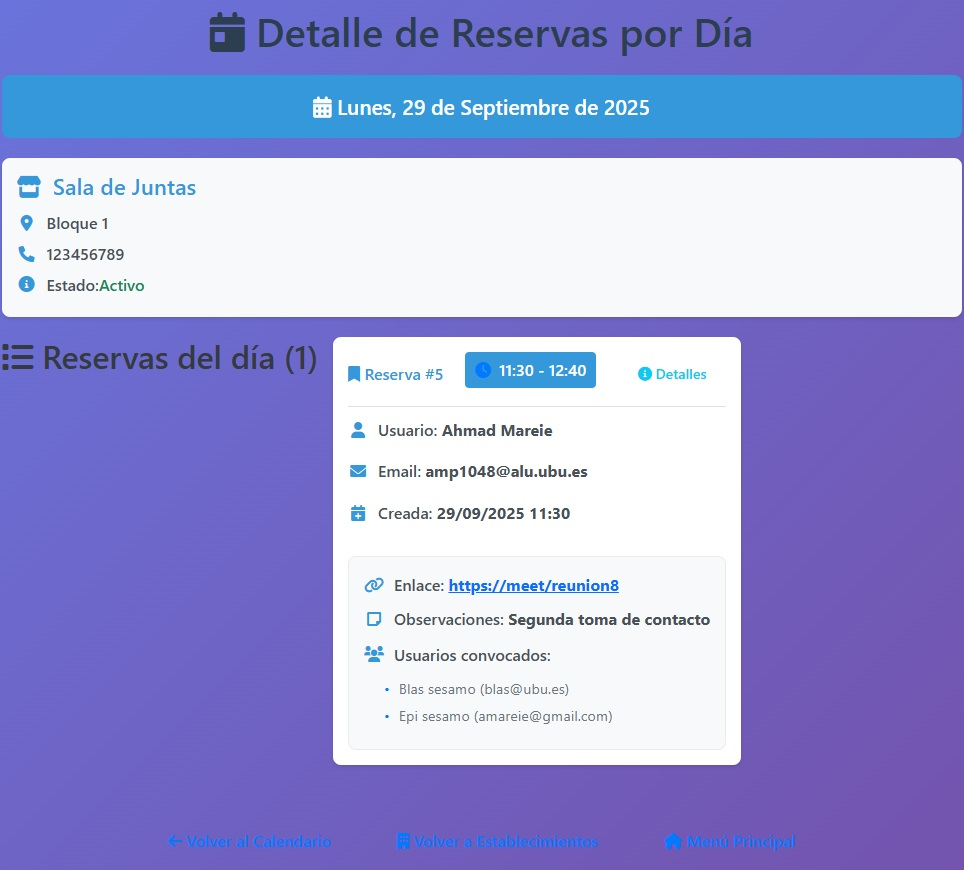
\includegraphics[width=0.5\linewidth]{reservapp_detalle_reservas}
	\caption{Detalle de una reserva particular.}
	\label{fig:reservapp_detalle_reservas}
\end{figure}

\begin{enumerate}
   \item \textbf{Lista de reservas del día}:
   \begin{itemize}
      \item Hora de cada reserva.
      \item Usuario que realizó la reserva.
      \item Información de contacto.
      \item Detalles de la convocatoria (si existe).
   \end{itemize}
   \item \textbf{Gestión de reservas}:
   \begin{itemize}
      \item Visualización completa de todas las reservas.
      \item Información de usuarios convocados.
      \item Enlaces de reunión y observaciones.
   \end{itemize}
\end{enumerate}

\subsection{Resolución de problemas comunes}

\begin{itemize}
   \item \textbf{Problemas de Acceso}:
   \begin{itemize}
      \item No puedo iniciar sesión:
      \begin{itemize}
         \item Verificar que el ID de usuario y contraseña sean correctos.
         \item Comprobar que la cuenta no esté bloqueada.
         \item Contactar con el administrador si persiste el problema.
      \end{itemize}
      \item He olvidado mi contraseña:
      \begin{itemize}
         \item Contactar con el administrador del sistema para restablecer la contraseña.
         \item El administrador puede asignar una contraseña temporal.
      \end{itemize}
   \end{itemize}

   \item \textbf{Problemas con Reservas}:
   \begin{itemize}
      \item No puedo crear una reserva:
      \begin{itemize}
         \item Verificar que el establecimiento esté activo.
         \item Comprobar que la fecha y hora estén dentro de los horarios de apertura.
         \item Verificar que no se haya alcanzado el aforo máximo.
         \item Asegurarse de que la hora de fin sea posterior a la hora de inicio.
      \end{itemize}
      \item No veo mis reservas:
      \begin{itemize}
         \item Verificar que esté accediendo al establecimiento correcto.
         \item Comprobar que tenga permisos para el establecimiento.
         \item Las reservas muy antiguas pueden no mostrarse por defecto.
      \end{itemize}
      \item Error al modificar una reserva:
      \begin{itemize}
         \item Solo se pueden modificar reservas futuras.
         \item Verificar que sea el propietario de la reserva.
         \item Comprobar la disponibilidad del nuevo horario solicitado.
      \end{itemize}
   \end{itemize}

   \item \textbf{Problemas con Convocatorias}:
   \begin{itemize}
      \item Los usuarios invitados no reciben emails:
      \begin{itemize}
         \item Verificar que las direcciones de email sean correctas.
         \item Comprobar las carpetas de spam/correo no deseado.
         \item Contactar con el administrador para verificar la configuración del servidor de correo.
      \end{itemize}
      \item No puedo encontrar usuarios para invitar:
      \begin{itemize}
         \item Verificar que esté escribiendo al menos 2 caracteres.
         \item Comprobar que los usuarios existan en el sistema.
         \item Los usuarios bloqueados pueden no aparecer en los resultados.
      \end{itemize}
   \end{itemize}

   \item \textbf{Problemas de Rendimiento}:
   \begin{itemize}
      \item La aplicación carga lentamente:
      \begin{itemize}
         \item Verificar la conexión a internet.
         \item Limpiar la caché del navegador.
         \item Contactar con el administrador si el problema persiste.
      \end{itemize}
      \item Los horarios no se cargan:
      \begin{itemize}
         \item Verificar que haya seleccionado una fecha válida.
         \item Comprobar que el establecimiento tenga horarios configurados.
         \item Refrescar la página si el problema persiste.
      \end{itemize}
   \end{itemize}
\end{itemize}

\apendice{Anexo de sostenibilización curricular}

\section{Introducción}
Este documento es una reflexión sobre cómo la sostenibilidad se integró en el proyecto ``ReservApp'', mi trabajo de fin de grado. Siguiendo las recomendaciones de la CRUE~\cite{crue}, la ``sostenibilización curricular'' no solo trata temas del medio ambiente, sino que busca un enfoque completo que incluya aspectos sociales, económicos y ambientales.

Aquí explico cómo un proyecto tecnológico como ReservApp me ayudó a desarrollar y aplicar estas competencias. El objetivo es mostrar cómo mi trabajo contribuye a formar un profesional más consciente de los desafíos globales y alineado con los Objetivos de Desarrollo Sostenible (ODS) de la ONU.

A lo largo de las siguientes secciones, analizaré el proyecto desde tres ángulos: social, económico y ambiental. Mostraré cómo las decisiones de diseño, la arquitectura y las funciones de la aplicación se conectan con los principios de la sostenibilidad.

\subsection{Sostenibilidad Social}
La \textbf{sostenibilidad social} trata de cuidar a las personas, la equidad y la armonía en una comunidad. Aunque una app de reservas parezca algo simple, ReservApp tiene un impacto directo aquí porque gestiona cómo la gente accede a los recursos de un lugar, como una universidad.

Uno de los aspectos destacables en este sentido es que el proyecto promueve la \textbf{equidad y la transparencia}. Al ofrecer un sistema único para todos, asegura que el acceso a espacios como salas de estudio sea justo y sin favoritismos. Esto evita confusiones y conflictos, creando un ambiente más tranquilo y equitativo. Básicamente, todos tienen las mismas oportunidades, y eso es importante para que la comunidad funcione bien.

Además, desarrollar esta aplicación me dio la oportunidad de aprender a \textbf{usar la tecnología para un fin social}. No se trataba de construir algo por construir, sino de resolver un problema real. Aprendí a entender las necesidades de la gente, a diseñar pensando en el usuario y a ver cómo la tecnología puede influir positivamente en las interacciones humanas. Al hacer la vida más fácil y organizada para estudiantes y personal, la aplicación mejora sutilmente su bienestar y el ambiente general.

\subsection{Sostenibilidad Económica}
La \textbf{sostenibilidad económica} busca ser eficiente e inteligente para no malgastar recursos valiosos. En un proyecto de software como ReservApp, esto se ve de varias maneras.

Por un lado, la aplicación ayuda a \textbf{optimizar el uso de los espacios físicos}. La aplicación ayuda a usar de forma más eficiente los recursos físicos. Las infraestructuras como aulas, laboratorios y equipos son muy caras de comprar y mantener. Un sistema como ReservApp se asegura de que estos recursos se usen al máximo, evitando que queden vacíos por falta de organización. Al optimizar su uso, la institución puede ahorrar mucho dinero al no tener que invertir en nuevas instalaciones.

Además, el proyecto se construyó con \textbf{tecnologías de código abierto (Open Source)} como Java, el \emph{framework} Spring y la base de datos MySQL. Esta decisión eliminó por completo los costos de licencias de software, lo que representa un modelo de desarrollo sostenible. Al usar este tipo de tecnologías, no solo aprovechamos un ecosistema robusto mantenido por una comunidad global, sino que también nos aseguramos de que el proyecto sea viable a largo plazo sin depender de empresas privadas con modelos de negocio restrictivos. Y no menos importante, las habilidades que adquirí con estas herramientas son un valor añadido que me acompañará en mi carrera profesional.

\subsection{Sostenibilidad Ambiental}
Aunque la \textbf{sostenibilidad ambiental} en un proyecto de software no siempre es obvia, su impacto es muy real. Se trata de usar menos energía y recursos para reducir nuestra huella ecológica.

El principal beneficio ambiental de ReservApp es la \textbf{reducción del uso de recursos materiales}. Al digitalizar el proceso de reserva, se elimina la necesidad de sistemas basados en papel como registros y formularios. El impacto de una sola hoja es pequeño, pero en el contexto de una institución grande, el ahorro acumulado de papel, tinta y los recursos de producción es significativo.

Además, de manera indirecta, la optimización en la gestión de espacios también contribuye al medio ambiente. Un uso más eficiente de las salas permite una mejor gestión de los recursos energéticos. Por ejemplo, al conocer la ocupación de los espacios, se puede optimizar la climatización y la iluminación, evitando el derroche de energía en áreas que no están en uso.

Por último, el propio diseño del software es un factor de sostenibilidad. La elección de una arquitectura optimizada no solo mejora el rendimiento de la aplicación, sino que también reduce la carga de trabajo de los servidores. Esto se traduce en un menor consumo energético en los centros de datos, lo cual tiene un impacto positivo en el medio ambiente.

\subsection{Conclusión}
Con "ReservApp" descubrí que el desarrollo de software va mucho más allá de la codificación. Fue un proyecto que me enseñó a aplicar mis conocimientos para diseñar soluciones que consideren la sostenibilidad en todas sus facetas.

A través de este trabajo, aprendí a crear soluciones tecnológicas que no solo funcionan bien, sino que también son justas para las personas, viables económicamente y respetuosas con el medio ambiente. Creo que esta visión es esencial para afrontar los desafíos del siglo XXI y para que, como ingenieros de software, podamos aportar nuestro granito de arena a un futuro más sostenible.


\bibliographystyle{plain}
\bibliography{bibliografiaAnexos}

\end{document}
